%%%%%%%%%%%%%%%%%%%%%%%%%%%%%%%%%%%%%%%%%%%%%%%%%%%%%%%%%%%%%%%%%%%%%%%%%%%%%%

\documentclass[unknownkeysallowed,11pt]{beamer}

%%%%%%%%%%%%%%%%%%%%%%%%%%%%%%%%%%%%%%%%%%%%%%%%%%%%%%%%%%%%%%%%%%%%%%%%%%%%%%

\usetheme{Boadilla}
\usefonttheme{serif}
\usecolortheme{default}

%%%%%%%%%%%%%%%%%%%%%%%%%%%%%%%%%%%%%%%%%%%%%%%%%%%%%%%%%%%%%%%%%%%%%%%%%%%%%%

\usepackage{euler,palatino}
\usepackage{amsmath,amssymb}
\usepackage[utf8]{inputenc}
\usepackage{xxcolor}
\usepackage{graphicx}
\usepackage[ruled]{algorithm2e}
\usepackage[english]{babel}
\usepackage{rotate}
\usepackage{shuffle}
\usepackage{minted}
\usepackage{url}
\usepackage{etoolbox}
\usepackage{tikz}
\usepackage{rotating}
\usetikzlibrary{snakes}
\usetikzlibrary{trees}
\usetikzlibrary{arrows}
\usetikzlibrary{matrix}

%%%%%%%%%%%%%%%%%%%%%%%%%%%%%%%%%%%%%%%%%%%%%%%%%%%%%%%%%%%%%%%%%%%%%%%%%%%%%%

\usepackage{csquotes}
\usepackage{breakcites}
\usepackage{hyperref}
\usepackage[autocite=superscript,
            sortcites,
            maxcitenames=3,
            doi=false,
            isbn=false,
            note=false,
            url=false,
            bibstyle=authoryear,
            style=authoryear,
            backend=bibtex]{biblatex}

\AtEveryCitekey{%
    \clearfield{title}%
    \clearfield{note}%
    \clearfield{pages}%
    \clearlist{location}%
    \clearlist{publisher}%
    \clearname{editor}%
}% end AtEveryCitekey

\bibliography{biblio.bib}
\renewcommand*{\multicitedelim}{\\}
\renewcommand{\footfullcite}[1]{\footnote[frame]{\fullcite{#1}}}
\def\bibfont{\tiny}
\beamertemplatenavigationsymbolsempty

%%%%%%%%%%%%%%%%%%%%%%%%%%%%%%%%%%%%%%%%%%%%%%%%%%%%%%%%%%%%%%%%%%%%%%%%%%%%%%

\newcommand{\PET}{pet}
\newcommand{\SBL}{sbl}

%%%%%%%%%%%%%%%%%%%%%%%%%%%%%%%%%%%%%%%%%%%%%%%%%%%%%%%%%%%%%%%%%%%%%%%%%%%%%%

\definecolor{Vert}{RGB}{20,100,20}
\setbeamercolor{title}{fg=Vert}
\setbeamercolor{frametitle}{fg=Vert}
\setbeamercolor{structure}{fg=Vert}

%%%%%%%%%%%%%%%%%%%%%%%%%%%%%%%%%%%%%%%%%%%%%%%%%%%%%%%%%%%%%%%%%%%%%%%%%%%%%%

\setbeamercovered{dynamic}

%%%%%%%%%%%%%%%%%%%%%%%%%%%%%%%%%%%%%%%%%%%%%%%%%%%%%%%%%%%%%%%%%%%%%%%%%%%%%%

%%% 
%%% complexity.tex
%%% 

\usepackage{xspace}

%%% ----------------------------------------------------------------------
%%% complexity classes
%%% ----------------------------------------------------------------------

% TIME
\newcommand{\DTIMEX}{{\sf\bf DTIME}}
\newcommand{\DTIMEclass}{\DTIMEX\xspace}
\newcommand{\DTIME}{\DTIMEclass}
% NL class
\newcommand{\NLclassbase}{{\sf\bf NL}}
\newcommand{\NLclass}{\NLclassbase\xspace}
% P class
\newcommand{\Pclassbase}{{\sf\bf P}}
\newcommand{\Pclass}{\Pclassbase\xspace}
% NP class
\newcommand{\NPclassbase}{{\sf\bf NP}}
\newcommand{\NPclass}{\NPclassbase\xspace}
% coNP class
\newcommand{\coNPclassbase}{{\sf\bf coNP}}
\newcommand{\coNPclass}{\coNPclassbase\xspace}
% PSPACE class
\newcommand{\PSPACEclassbase}{{\sf\bf PSPACE}}
\newcommand{\PSPACEclass}{\PSPACEclassbase\xspace}
% MAXSNP class
\newcommand{\MaxSNPclassbase}{{\sf\bf MaxSNP}}
\newcommand{\MaxSNPclass}{\MaxSNPclassbase\xspace}
% MAXNP class
\newcommand{\MaxNPclassbase}{{\sf\bf MaxNP}}
\newcommand{\MaxNPclass}{\MaxNPclassbase\xspace}
% EPTAS class
\newcommand{\EPTASclassbase}{{\sf\bf EPTAS}}
\newcommand{\EPTASclass}{\EPTASclassbase\xspace}
% FPTAS class
\newcommand{\FPTASclassbase}{{\sf\bf FPTAS}}
\newcommand{\FPTASclass}{\FPTASclassbase\xspace}
% PTAS class
\newcommand{\PTASclassbase}{{\sf\bf PTAS}}
\newcommand{\PTASclass}{\PTASclassbase\xspace}
% APX class
\newcommand{\APXclassbase}{{\sf\bf APX}}
\newcommand{\APXclass}{\APXclassbase\xspace}
% log-APX class
\newcommand{\logAPXclassbase}{{\sf\bf log{\tt -}APX}}
\newcommand{\logAPXclass}{\logAPXclassbase\xspace}
% poly-APX class
\newcommand{\polyAPXclassbase}{{\sf\bf poly{\tt -}APX}}
\newcommand{\polyAPXclass}{\polyAPXclassbase\xspace}
% exp-APX class
\newcommand{\expAPXclassbase}{{\sf\bf exp{\tt -}APX}}
\newcommand{\expAPXclass}{\expAPXclassbase\xspace}
% NPO class
\newcommand{\NPOclassbase}{{\sf\bf NPO}}
\newcommand{\NPOclass}{\NPOclassbase\xspace}
% #P class
\newcommand{\sharpPclassbase}{\#{\sf\bf P}}
\newcommand{\sharpPclass}{\sharpPclassbase\xspace}
% FPT class
\newcommand{\FPTclassbase}{{\sf\bf FPT}}
\newcommand{\FPTclass}{\FPTclassbase\xspace}
% W class
\newcommand{\Wclassbase}[1]{{\sf\bf W[#1]}}
\newcommand{\Wclass}[1]{\Wclassbase{#1}\xspace}
% W class
\newcommand{\XPclassbase}{{\sf\bf XP}}
\newcommand{\XPclass}{\XPclassbase\xspace}
% WNL class
\newcommand{\WNLclassbase}{{\sf\bf WNL}}
\newcommand{\WNLclass}{\WNLclassbase\xspace}
% ZPP class
\newcommand{\ZPPclassbase}{{\sf\bf ZPP}}
\newcommand{\ZPPclass}{\ZPPclassbase\xspace}
% NPK class
\newcommand{\NPKclassbase}{{\sf\bf NPK}}
\newcommand{\NPKclass}{\NPKclassbase\xspace}
\newcommand{\NPKandclass}{\text{$\NPKclass_\text{and}$}\xspace}
\newcommand{\NPKzeroandclass}{\text{$\NPKclass^0_\text{and}$}\xspace}
\newcommand{\NPKorclass}{\text{$\NPKclass_\text{or}$}\xspace}
\newcommand{\NPKzeroorclass}{\text{$\NPKclass^0_\text{or}$}\xspace}

%%% ----------------------------------------------------------------------
%%% complete
%%% ----------------------------------------------------------------------

% keyword
\newcommand{\complete}{\text{-complete}}
% NL-complete
\newcommand{\NLcomplete}{\NLclassbase\complete\xspace}
\newcommand{\NLC}{\NLcomplete}
% P-complete
\newcommand{\Pcomplete}{\Pclassbase\complete\xspace}
\newcommand{\PC}{\Pcomplete}
% NP-complete
\newcommand{\NPcomplete}{\NPclassbase\complete\xspace}
\newcommand{\NPC}{\NPcomplete}
% coNP-complete
\newcommand{\coNPcomplete}{\coNPclassbase\complete\xspace}
\newcommand{\coNPC}{\coNPcomplete}
% PSPACE-complete
\newcommand{\PSPACEcomplete}{\PSPACEclassbase\complete\xspace}
\newcommand{\PSPACEC}{\PSPACEcomplete}
% MAXSNP-complete
\newcommand{\MaxSNPcomplete}{\MaxSNPclassbase\complete\xspace}
\newcommand{\MaxSNPC}{\MaxSNPcomplete}
% APX-complete
\newcommand{\APXcomplete}{\APXclassbase\complete\xspace}
\newcommand{\APXC}{\APXcomplete}
% #P-complete
\newcommand{\sharpPcomplete}{\sharpPclassbase\complete\xspace}
\newcommand{\sharpPC}{\sharpPcomplete}
% W[i]-complete
\newcommand{\Wcomplete}[1]{\Wclassbase{#1}\complete\xspace}
\newcommand{\WC}[1]{\Wcomplete{#1}}
% WNL-complete
\newcommand{\WNLcomplete}{\WNLclassbase\complete\xspace}
\newcommand{\WNLC}{\WNLcomplete}

%%% ----------------------------------------------------------------------
%%% hard
%%% ----------------------------------------------------------------------

% keyword
\newcommand{\hard}{\text{-hard}}
% NL-hard
\newcommand{\NLhard}{\NLclassbase\hard\xspace}
\newcommand{\NLH}{\NLhard}
% P-hard
\newcommand{\Phard}{\NPclassbase\hard\xspace}
\newcommand{\PH}{\Phard}
% NP-hard
\newcommand{\NPhard}{\NPclassbase\hard\xspace}
\newcommand{\NPH}{\NPhard}
% coNP-hard
\newcommand{\coNPhard}{\coNPclassbase\hard\xspace}
\newcommand{\coNPH}{\coNPhard}
% PSPACE-hard
\newcommand{\PSPACEhard}{\PSPACEclassbase\hard\xspace}
\newcommand{\PSPACEH}{\PSPACEhard}
% MAXSNP-hard
\newcommand{\MaxSNPhard}{\MaxSNPclassbase\hard\xspace}
\newcommand{\MaxSNPH}{\MaxSNPhard}
% APX-hard
\newcommand{\APXhard}{\APXclassbase\hard\xspace}
\newcommand{\APXH}{\APXhard}
% WNL-hard
\newcommand{\WNLhard}{\WNLclassbase\hard\xspace}
\newcommand{\WNLH}{\WNLhard}
% #P-hard
\newcommand{\sharpPhard}{\sharpPclassbase\hard\xspace}
\newcommand{\sharpPH}{\sharpPhard}
% W[i]-hard
\newcommand{\Whard}[1]{\Wclassbase{#1}\hard\xspace}
\newcommand{\WH}[1]{\Whard{#1}}

%%% ----------------------------------------------------------------------
%%% hardness
%%% ----------------------------------------------------------------------

% keyword
\newcommand{\hardness}{\text{-hardness}}
% NP-hardness
\newcommand{\NPhardness}{\NPclassbase\hardness\xspace}
% APX-hardness
\newcommand{\APXhardness}{\APXclassbase\hardness\xspace}
% W[i]-hardness
\newcommand{\Whardness}[1]{\Wclassbase{#1}\hardness\xspace}
% WNL-hardness
\newcommand{\WNLhardness}{\WNLclassbase\hardness\xspace}

%%% ----------------------------------------------------------------------
%%% completeness
%%% ----------------------------------------------------------------------

% keyword
\newcommand{\completeness}{\text{-completeness}}
% NL-completeness
\newcommand{\NLcompleteness}{\NLclassbase\completeness\xspace}
% P-completeness
\newcommand{\Pcompleteness}{\NPclassbase\completeness\xspace}
% NP-completeness
\newcommand{\NPcompleteness}{\NPclassbase\completeness\xspace}
% APX-completeness
\newcommand{\APXcompleteness}{\APXclassbase\completeness\xspace}
% #P-completeness
\newcommand{\sharpPcompleteness}{\sharpPclassbase\completeness\xspace}
% W[i]-hard
\newcommand{\Wcompleteness}[1]{\W{#1}-\completeness\xspace}

%%% ----------------------------------------------------------------------
%%% reduction
%%% ----------------------------------------------------------------------

\newcommand{\reduction}{reduction}
\newcommand{\reductions}{reductions}
\newcommand{\reductible}{reductible}

\newcommand{\APTypeReduction}{AP}
\newcommand{\PTASTypeReduction}{PTAS}
\newcommand{\LTypeReduction}{L}
\newcommand{\ETypeReduction}{E}
\newcommand{\fptTypeReduction}{fpt}
\newcommand{\pptTypeReduction}{ptp}

% AP-reduction
\newcommand{\APreduction}{\APTypeReduction-\reduction\xspace}
\newcommand{\APreductions}{\APTypeReduction-\reductions\xspace}
\newcommand{\APreductible}{\APTypeReduction-\reductible\xspace}

% PTAS-reduction
\newcommand{\PTASeduction}{\PTASTypeReduction-\reduction\xspace}
\newcommand{\PTASreductions}{\PTASTypeReduction-\reductions\xspace}
\newcommand{\PTASreductible}{\PTASTypeReduction-\reductible\xspace}

% L-reduction
\newcommand{\Lreduction}{\LTypeReduction-\reduction\xspace}
\newcommand{\Lreductions}{\LTypeReduction-\reductions\xspace}
\newcommand{\Lreductible}{\LTypeReduction-\reductible\xspace}

% E-reduction
\newcommand{\Ereduction}{\ETypeReduction-\reduction\xspace}
\newcommand{\Ereductions}{\ETypeReduction-\reductions\xspace}
\newcommand{\Ereductible}{\ETypeReduction-\reductible\xspace}

% fpt-reduction
\newcommand{\fptreduction}{\fptTypeReduction-\reduction\xspace}
\newcommand{\fptreductions}{\fptTypeReduction-\reductions\xspace}
\newcommand{\fptreductible}{\fptTypeReduction-\reductible\xspace}

% ptp-reduction
\newcommand{\ptpreduction}{\ptpTypeReduction-\reduction\xspace}
\newcommand{\ptpreductions}{\ptpTypeReduction-\reductions\xspace}
\newcommand{\ptpreductible}{\ptpTypeReduction-\reductible\xspace}

% symbols
\DeclareMathOperator{\APreduce}{\text{$\leq_{\text{\APTypeReduction}}$}}
\DeclareMathOperator{\PTASreduce}{\text{$\leq_{\text{\PTASTypeReduction}}$}}
\DeclareMathOperator{\Lreduce}{\text{$\leq_{\text{\LTypeReduction}}$}}
\DeclareMathOperator{\Ereduce}{\text{$\leq_{\text{\ETypeReduction}}$}}
\DeclareMathOperator{\fptreduce}{\text{$\leq_{\text{\fptTypeReduction}}$}}
\DeclareMathOperator{\ptpreduce}{\text{$\leq_{\text{\fptTypeReduction}}$}}

%% 
%% Approximation
%%
\DeclareMathOperator{\poly}{poly}
\DeclareMathOperator{\POLY}{poly}
\DeclareMathOperator{\SIZE}{size}
\newcommand{\sol}{{\sf sol}\xspace}
\newcommand{\PB}[1]{\textsf{\scshape{#1}}}
\newcommand{\OPTname}{opt}
\newcommand{\OPT}{\text{$\mathsf{\bf \OPTname}$}}
\newcommand{\OPTpb}[1]{\text{$\mathsf{\OPTname}_{\PB{#1}}$}}
\newcommand{\ALGO}[1]{\textbf{\ttfamily\sf #1}}
\newcommand{\Approxname}{Approx}
\newcommand{\APPROX}[1]{\text{$\ALGO{\Approxname}_{\,\PB{#1}}$}}
\newcommand{\PCP}{{\sf\bf PCP}\xspace}

%%
%% Problem Definition
%%
\newcommand{\PbDef}[3]{%
\begin{center}
  \begin{tabular}{l}%
    \shadowbox{%
    \begin{minipage}[c]{.9\textwidth}
      \smallskip%
      \par\noindent%
      {#1}%
      \smallskip
      \par\noindent%
      $\bullet$
      \textbf{\textsf{Input}}~: #2% 
      \medskip
      \par\noindent%
      $\bullet$
      \textbf{\textsf{Question}}~:
      #3% 
      \smallskip%
      \par\noindent%
    \end{minipage}
  }% end shadowbox
  \end{tabular}%
\end{center}
}%
\newcommand{\PbDefinition}{\PbDef}

%%
%% Problem (Input + Output) Definition
%%
\newcommand{\PbInputOutputDef}[3]{%
\begin{center}
  \begin{tabular}{l}%
    \shadowbox{%
    \begin{minipage}[c]{.9\textwidth}
      \smallskip%
      \par\noindent%
      \PB{#1}%
      \medskip%
      \par\noindent%
      $\bullet$
      \textbf{\textsf{Input}}~: #2% 
      \medskip
      \par\noindent%
      $\bullet$
      \textbf{\textsf{Output}}~:
      #3% 
      \smallskip%
      \par\noindent%
    \end{minipage}
  }% end shadowbox
  \end{tabular}%
\end{center}
}%
\newcommand{\PbInputOutputDefinition}{\PbInputOutputDef}


%%
%% Optimization Problem Definition
%%

\newcommand{\OptPbDefinition}[4]{%
\begin{center}
  \begin{tabular}{l}%
    \shadowbox{%
    \begin{minipage}[c]{.9\textwidth}
      \par\noindent%
      \shadowbox{#1}%
      \par\noindent%
      $\bullet$
      \textbf{\textsf{Input}}~: #2% 
      \par\noindent%
      $\bullet$
      \textbf{\textsf{Solution}}~: #3%  
      \par\noindent%
      $\bullet$
      \textbf{\textsf{Measure}}~: #4% 
      \par\noindent%
    \end{minipage}
    }% end shadowbox
  \end{tabular}%
\end{center}
}%

%%
%% Parameterized Problem Definition
%%
\newcommand{\ParamPbDefinition}[4]{%
\begin{center}
  \begin{tabular}{l}%
    %\shadowbox{%
    \begin{minipage}[c]{.95\textwidth}
      % \smallskip%
      \par\noindent%
      #1%
      % \smallskip%
      \par\noindent%
      \textbf{\textsf{Input}}~: #2% 
      % \smallskip
      \par\noindent%
      \textbf{\textsf{Question}}~: #3%  
      % \smallskip
      \par\noindent%
      \textbf{\textsf{Parameter}}~: #4% 
      %\smallskip%
      \par\noindent%
    \end{minipage}
  %}% end shadowbox
  \end{tabular}%
\end{center}
}%
\newcommand{\ParamPbDefinitionTwo}[5]{%
\begin{center}
  \begin{tabular}{l}%
    \shadowbox{%
    \begin{minipage}[c]{.9\textwidth}
      \smallskip%
      \par\noindent%
      \shadowbox{#1}%
      \medskip%
      \par\noindent%
      $\bullet$
      \textbf{\textsf{Input}}~: #2% 
%      \medskip
      \par\noindent%
      $\bullet$
      \textbf{\textsf{Parameter}}~: #3% 
 %     \medskip
      \par\noindent%
      $\bullet$
      \textbf{\textsf{Parameter}}~: #4% 
      \medskip
      \par\noindent%
      $\bullet$
      \textbf{\textsf{Question}}~: #5%  
      \smallskip%
      \par\noindent%
    \end{minipage}
    }% end shadowbox
  \end{tabular}%
\end{center}
}%
\newcommand{\ParamPbDefinitionThree}[6]{%
\begin{center}
  \begin{tabular}{l}%
    \shadowbox{%
    \begin{minipage}[c]{.9\textwidth}
      \smallskip%
      \par\noindent%
      \shadowbox{#1}%
      \medskip%
      \par\noindent%
      $\bullet$
      \textbf{\textsf{Input}}~: #2% 
%      \medskip
      \par\noindent%
      $\bullet$
      \textbf{\textsf{Parameter}}~: #3% 
%      \medskip
      \par\noindent%
      $\bullet$
      \textbf{\textsf{Parameter}}~: #4% 
%      \medskip
      \par\noindent%
      $\bullet$
      \textbf{\textsf{Parameter}}~: #5%  
      \medskip
      \par\noindent%
      $\bullet$
      \textbf{\textsf{Question}}~: #6%  
      \smallskip%
      \par\noindent%
    \end{minipage}
    }% end shadowbox
  \end{tabular}%
\end{center}
}%
\newcommand{\ParamPbDefinitionFour}[7]{%
\begin{center}
  \begin{tabular}{l}%
    \shadowbox{%
    \begin{minipage}[c]{.9\textwidth}
      \smallskip%
      \par\noindent%
      \shadowbox{#1}%
      \medskip%
      \par\noindent%
      $\bullet$
      \textbf{\textsf{Input}}~: #2% 
%      \medskip
      \par\noindent%
      $\bullet$
      \textbf{\textsf{Parameter}}~: #3% 
%      \medskip
      \par\noindent%
      $\bullet$
      \textbf{\textsf{Parameter}}~: #4% 
%      \medskip
      \par\noindent%
      $\bullet$
      \textbf{\textsf{Parameter}}~: #5%  
%      \medskip
      \par\noindent%
    $\bullet$
      \textbf{\textsf{Parameter}}~: #6%  
      \medskip
      \par\noindent%
      $\bullet$
      \textbf{\textsf{Question}}~: #7%  
      \smallskip%
      \par\noindent%
    \end{minipage}
    }% end shadowbox
  \end{tabular}%
\end{center}
}%
\newcommand{\ParamPbDefinitionFive}[8]{%
\begin{center}
  \begin{tabular}{l}%
    \shadowbox{%
    \begin{minipage}[c]{.9\textwidth}
      \smallskip%
      \par\noindent%
      \shadowbox{#1}%
      \medskip%
      \par\noindent%
      $\bullet$
      \textbf{\textsf{Input}}~: #2% 
%      \medskip
      \par\noindent%
      $\bullet$
      \textbf{\textsf{Parameter}}~: #3% 
%      \medskip
      \par\noindent%
      $\bullet$
      \textbf{\textsf{Parameter}}~: #4% 
%      \medskip
      \par\noindent%
      $\bullet$
      \textbf{\textsf{Parameter}}~: #5%  
%      \medskip
      \par\noindent%
    $\bullet$
      \textbf{\textsf{Parameter}}~: #6%  
%      \medskip
      \par\noindent%
    $\bullet$
      \textbf{\textsf{Parameter}}~: #7%  
      \medskip
      \par\noindent%
      $\bullet$
      \textbf{\textsf{Question}}~: #8%  
      \smallskip%
      \par\noindent%
    \end{minipage}
    }% end shadowbox
  \end{tabular}%
\end{center}
}%
\newcommand{\ParamPbDefinitionSix}[9]{%
\begin{center}
  \begin{tabular}{l}%
    \shadowbox{%
    \begin{minipage}[c]{.9\textwidth}
      \smallskip%
      \par\noindent%
      \shadowbox{#1}%
      \medskip%
      \par\noindent%
      $\bullet$
      \textbf{\textsf{Input}}~: #2% 
%      \medskip
      \par\noindent%
      $\bullet$
      \textbf{\textsf{Parameter}}~: #3% 
%      \medskip
      \par\noindent%
      $\bullet$
      \textbf{\textsf{Parameter}}~: #4% 
%      \medskip
      \par\noindent%
      $\bullet$
      \textbf{\textsf{Parameter}}~: #5%  
%      \medskip
      \par\noindent%
      $\bullet$
      \textbf{\textsf{Parameter}}~: #6%  
%      \medskip
      \par\noindent%
      $\bullet$
      \textbf{\textsf{Parameter}}~: #7%  
%      \medskip
      \par\noindent%
      $\bullet$
      \textbf{\textsf{Parameter}}~: #8%  
      \medskip
      \par\noindent%
      $\bullet$
      \textbf{\textsf{Question}}~: #9%  
      \smallskip%
      \par\noindent%
    \end{minipage}
    }% end shadowbox
  \end{tabular}%
\end{center}
}%



\input{graph}
\input{matrix}

%%%%%%%%%%%%%%%%%%%%%%%%%%%%%%%%%%%%%%%%%%%%%%%%%%%%%%%%%%%%%%%%%%%%%%%%%%%%%%

\title[Permutation Equivelent Matrices]{%
  \textbf{Obtaining a Triangular Matrix by \\
  Independent Row-Column Permutations}
}

\subtitle{
    \textbf{St\'ephane~Vialette}\\
    Laboratoire d'Informatique Gaspard-Monge\\
    Université Paris-Est Marne-la-Vallée \\
    UMR CNRS 8049 \\
    ~\\
    
\includegraphics[width=1.cm,height=1.25cm,keepaspectratio]{logos/CNRSfr}
    \qquad
    
\includegraphics[width=1.cm,height=1.25cm,keepaspectratio]{logos/ecole_ponts_RVB300.jpg}
    \qquad
    
\includegraphics[width=1.5cm,height=2cm,keepaspectratio]{logos/LIGM}
    \qquad
    \raisebox{.25cm}{
\includegraphics[width=1.cm,height=1.25cm,keepaspectratio]{logos/LogoEsieeParis}}
    \qquad
    \raisebox{.25cm}{
\includegraphics[width=1.cm,height=1.25cm,keepaspectratio]{logos/UPEM_LOGO_EDITION}}
}

\author[Fertin, Rusu and V.]{
    \textbf{Guillaume~Fertin}\quad\textbf{Irena~Rusu}\quad\textbf{S.~V}
}%

\date[ISAAC 15, Nagoya, Japan]{
    {
    \scriptsize 26th International Symposium on Algorithms and Computation \\ December 9-11, 2015
    }
}% end date

%%%%%%%%%%%%%%%%%%%%%%%%%%%%%%%%%%%%%%%%%%%%%%%%%%%%%%%%%%%%%%%%%%%%%%%%%%%%%%

\begin{document}

%%%%%%%%%%%%%%%%%%%%%%%%%%%%%%%%%%%%%%%%%%%%%%%%%%%%%%%%%%%%%%%%%%%%%%%%%%%%%%

\newcommand\mygrid[3][]{      % this definition uses \foreach inside a matrix
  \let\mymatrixcontent\empty  % see http://tex.stackexchange.com/q/60394/18228
  \newcommand{\row}{%
    \foreach \j in {1,...,#2}{
      \foreach \i in {1,...,#3} {%
        \begingroup\edef\x{\endgroup
           \noexpand\gappto\noexpand\mymatrixcontent{|[draw,minimum size=1cm,#1]| \&}}\x
        }%
      \gappto\mymatrixcontent{\\}%
    }
  }
  \row
  \matrix(m)[matrix of nodes,ampersand replacement=\&,row sep=-\pgflinewidth,column sep=-\pgflinewidth]{
    \mymatrixcontent
  };
  \foreach \x[count=\i from 0] in {1,...,#2}\node[left] at (m-\x-1.west) {$\i$};
  \foreach \y[count=\j from 0] in {1,...,#3}\node[above] at (m-1-\y.north) {$\j$};
}

%%%%%%%%%%%%%%%%%%%%%%%%%%%%%%%%%%%%%%%%%%%%%%%%%%%%%%%%%%%%%%%%%%%%%%%%%%%%%%

\frame{\titlepage}

%%%%%%%%%%%%%%%%%%%%%%%%%%%%%%%%%%%%%%%%%%%%%%%%%%%%%%%%%%%%%%%%%%%%%%%%%%%%%%

\begin{frame}
    \frametitle{Motivations}

    In his contribution to the tribute to the late Professor
    Erd\"os
    \texttt{\small(%
    H.~Wilf,
    \emph{Combinatorics, Geometry and Probability: A Tribute to Paul Erd{\"o}s},
    1997%
    )},
    Wilf posed the following question:

    \bigskip

    \begin{center}
      \begin{minipage}{.9\textwidth}
        %\centering
        \emph{
          ``Let $A$ be an $n \times n$ matrix of $0$'s and $1$'s. Consider the
          computational problem: do there exist permutations $P$ of the rows
          of $A$, and $Q$, of the columns of $A$ such that after carrying out
          these permutations, $A$ is triangular? The question we ask concerns
          the complexity of the problem.
          Is this problem \NPC?
          Or, does there exist a polynomial-time algorithm for doing it?''}
        \end{minipage}
    \end{center}
\end{frame}

%%%%%%%%%%%%%%%%%%%%%%%%%%%%%%%%%%%%%%%%%%%%%%%%%%%%%%%%%%%%%%%%%%%%%%%%%%%%%%

\begin{frame}
    \frametitle{Example}

    \begin{center}
      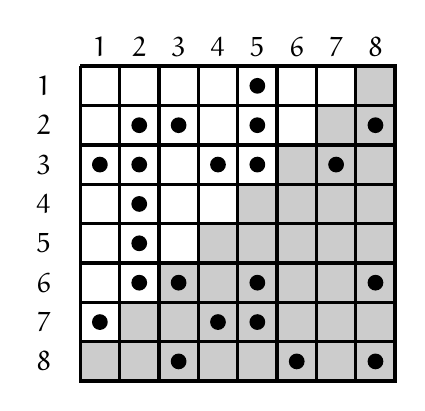
\begin{tikzpicture}[scale=0.5]
        \draw [shift={(0.5,0.5)},fill=black!20,very thick]
        (0,0) -- (0,1) -- (1,1) -- (1,2) -- (2,2) --
        (2,3) -- (3,3) -- (3,4) -- (4,4) -- (4,5) --
        (5,5) -- (5,6) -- (6,6) -- (6,7) -- (7,7) --
        (7,8) -- (8,8) -- (8,0) -- cycle;
        \draw[shift={(0.5,0.5)},very thick] (0,0) grid (8,8);
        \foreach \x in {1,2,...,8} {
          \node[left] at (0,9-\x) {$\x$};
        }
        \foreach \x in {1,2,...,8} {
          \node at (\x,9) {$\x$};
        }
        \foreach \x/\y in {%
          1/5,
          2/2, 2/3, 2/5, 2/8,
          3/1, 3/2, 3/4, 3/5, 3/7,
          4/2,
          5/2,
          6/2, 6/3, 6/5, 6/8,
          7/1, 7/4, 7/5,
          8/3, 8/6, 8/8} {
            \fill (\y,9-\x) circle(0.2);
        }
      \end{tikzpicture}
      \onslide<2>
      \qquad\qquad
      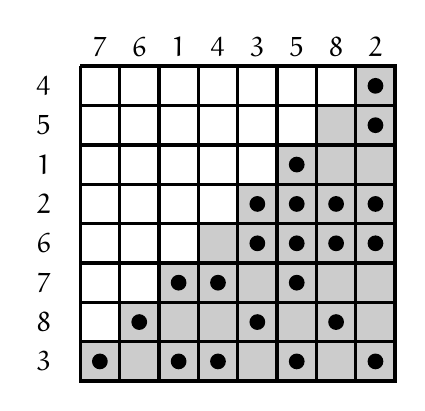
\begin{tikzpicture}[scale=0.5]
        \draw [shift={(0.5,0.5)},fill=black!20,very thick]
        (0,0) -- (0,1) -- (1,1) -- (1,2) -- (2,2) --
        (2,3) -- (3,3) -- (3,4) -- (4,4) -- (4,5) --
        (5,5) -- (5,6) -- (6,6) -- (6,7) -- (7,7) --
        (7,8) -- (8,8) -- (8,0) -- cycle;
        \draw[shift={(0.5,0.5)},very thick] (0,0) grid (8,8);
        \foreach \x/\l in {1/4, 2/5, 3/1, 4/2, 5/6, 6/7, 7/8, 8/3} {
          \node[left] at (0,9-\x) {$\l$};
        }
        \foreach \x/\l in {1/7, 2/6, 3/1, 4/4, 5/3, 6/5, 7/8, 8/2} {
          \node at (\x,9) {$\l$};
        }
        \foreach \x/\y in {%
          1/8,
          2/8,
          3/6,
          4/5, 4/6, 4/7, 4/8,
          5/5, 5/6, 5/7, 5/8,
          6/3, 6/4, 6/6,
          7/2, 7/5, 7/7,
          8/1, 8/3, 8/4, 8/6, 8/8} {
            \fill (\y,9-\x) circle(0.2);
        }
      \end{tikzpicture}
    \end{center}
\end{frame}


%%%%%%%%%%%%%%%%%%%%%%%%%%%%%%%%%%%%%%%%%%%%%%%%%%%%%%%%%%%%%%%%%%%%%%%%%%%%%%

\begin{frame}[fragile]
    \frametitle{Permutation-equivalent matrix}

    \begin{itemize}
      \item
      Write $\lrtm$ for the \textbf{full lower right triangular $(0,1)$-matrix}.

      \bigskip

      \item
      Let $A \leq \lrtm$ denote the fact that $A$ is lower right triangular.

      \medskip

      ($a_{i,j} = 0$ for $i+j \leq n$, $n$ is the order of the matrix.)

      \bigskip

      \item
      $A$ is \textbf{permutation-equivalent triangular} if there exist permutation matrices
      $P$ and $Q$ such that $PAQ \leq \lrtm$.

      \medskip

      (The orientation of the triangular
      matrix is of no importance.)
    \end{itemize}
\end{frame}

%%%%%%%%%%%%%%%%%%%%%%%%%%%%%%%%%%%%%%%%%%%%%%%%%%%%%%%%%%%%%%%%%%%%%%%%%%%%%%

\begin{frame}[fragile]
    \frametitle{Permanent}

    \begin{definition}
      % Let $A = [a_{i,j}]$ be square $(0,1)$-matrix of order $n$.
      %
      % \medskip
      %
      % The \textbf{permanent} of $A$ is defined as the number given by
      % the formula
      % $\PER(A) = \sum_{(j_1, j_2, \ldots, j_n) \in S_n}
      % a_{1,j_1}\,a_{2,j_2}\, \ldots a_{n,j_n}$,
      The \textbf{permanent} of an $n$-by-$n$ matrix $A = [a_{i,j}]$ is defined as
      $$
        \PER(A) = \sum_{\pi \in S_n} \prod_{i=1}^{n} a_{i, \pi(i)}\text{.}
      $$
      The sum here extends over all elements $\pi$ of the symmetric group
      $S_n$, \emph{i.e.} over all permutations of the numbers $1, 2, \ldots, n$.
    \end{definition}

    \begin{overprint}
      \onslide<1>
      \begin{exampleblock}{Example}
        $$
        \PER\left(
        \begin{bmatrix}
          1 & 0 & 0 & 1 \\
          1 & 0 & 0 & 1 \\
          0 & 1 & 1 & 0 \\
          1 & 1 & 1 & 1
        \end{bmatrix}
        \right)
        = 4
        $$
      \end{exampleblock}

      \onslide<2>
      \begin{itemize}
        \item
        Unlike the determinant, we do not put a minus sign in front of some of the terms in the
        summation.

        \medskip

        \item
        Computing $\PER(A)$ is \sharpPcomplete~
        \texttt{\small(L.~Valiant, 1979)}.

        \medskip

        \item
        Of particular importance,
        the permanent does not change if the rows or columns of A are permuted.
      \end{itemize}

      \onslide<3>
      \begin{theorem}[\texttt{\small R.A.~Brualdi and H.J.~Ryser, 1991}]
      $\PER(A)=1$ if and only if the lines of $A$
      may be permuted to yield a triangular matrix with $1$'s
      in the $n$ main diagonal positions and $0$'s above the main diagonal.
      \end{theorem}

      \onslide<4>
      \begin{theorem}
        If $A$ is a permutation-equivalent triangular matrix
        then $\PER(A) \leq 1$.
      \end{theorem}
    \end{overprint}

\end{frame}

%%%%%%%%%%%%%%%%%%%%%%%%%%%%%%%%%%%%%%%%%%%%%%%%%%%%%%%%%%%%%%%%%%%%%%%%%%%%%%

\begin{frame}
    \frametitle{Collection of subsets}

    \begin{center}
      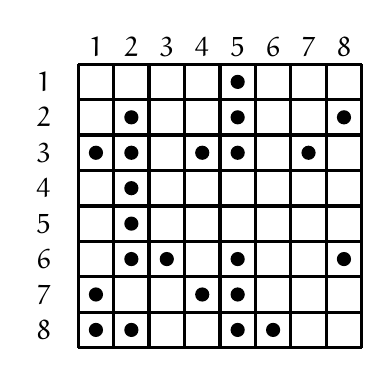
\begin{tikzpicture}[baseline={(current bounding box.center)},scale=0.45]
        % \draw [shift={(0.5,0.5)},fill=black!20,very thick]
        % (0,0) -- (0,1) -- (1,1) -- (1,2) -- (2,2) --
        % (2,3) -- (3,3) -- (3,4) -- (4,4) -- (4,5) --
        % (5,5) -- (5,6) -- (6,6) -- (6,7) -- (7,7) --
        % (7,8) -- (8,8) -- (8,0) -- cycle;
        \draw[shift={(0.5,0.5)},very thick] (0,0) grid (8,8);
        \foreach \x in {1,2,...,8} {
          \node[left] at (0,9-\x) {$\x$};
        }
        \foreach \x in {1,2,...,8} {
          \node at (\x,9) {$\x$};
        }
        \foreach \x/\y in {%
          1/5,
          2/2, 2/5, 2/8,
          3/1, 3/2, 3/4, 3/5, 3/7,
          4/2,
          5/2,
          6/2, 6/3, 6/5, 6/8,
          7/1, 7/4, 7/5,
          8/1, 8/2, 8/5, 8/6} {
            \fill (\y,9-\x) circle(0.2);
        }
      \end{tikzpicture}
      \quad
      \onslide<2->
      \begin{minipage}{.5\textwidth}
        \begin{align*}
          \mathcal{S} &= \{S_1, S_2, S_3, S_4, S_5, S_6, S_7, S_8\}
          \\
          S_i &\subseteq \{x_1, x_2, x_3, x_4, x_5, x_6, x_7, x_8\}
        \end{align*}
        \onslide<3>
        \begin{align*}
          S_1 &= \{x_5\} \\
          S_2 &= \{x_2, x_5, x_8\} \\
          S_3 &= \{x_1, x_2, x_4, x_5, x_7\} \\
          S_4 &= \{x_2\} \\
          S_5 &= \{x_2\} \\
          S_6 &= \{x_2, x_3, x_5, x_8\} \\
          S_7 &= \{x_1, x_4, x_5\} \\
          S_8 &= \{x_1, x_2, x_5, x_6\}
        \end{align*}
    \end{minipage}
    \end{center}
\end{frame}

%%%%%%%%%%%%%%%%%%%%%%%%%%%%%%%%%%%%%%%%%%%%%%%%%%%%%%%%%%%%%%%%%%%%%%%%%%%%%%

\begin{frame}
  \frametitle{Collection of subsets}

  \begin{definition}
    Let $\mathcal{S} = (S_i : 1 \leq i \leq n)$ be a configuration of subsets of some
    ground $n$-set $X$.

    A bijective mapping $\varphi : \mathcal{S} \to [n]$ is said to be a
    \textbf{stepwise bounded labeling} (or \textbf{\SBL} for short) of $\mathcal{S}$ if
    $\left|\bigcup_{\varphi(S_j) \leq i}S_j\right| \leq i$
    for $1 \leq i \leq n$.
  \end{definition}

  \bigskip

  \begin{lemma}
      Let $\mathcal{S} = (S_i : 1 \leq i \leq n)$ be a configuration of subsets of
      some ground $n$-set, and let $A$ be the corresponding incidence matrix.
      There exist permutation matrices $P$ and $Q$ of order $n$
      such that $PAQ \leq \lrtm_{\,n}$ if and only if
      there exists an \SBL\ of $\mathcal{S}$.
  \end{lemma}
\end{frame}

%%%%%%%%%%%%%%%%%%%%%%%%%%%%%%%%%%%%%%%%%%%%%%%%%%%%%%%%%%%%%%%%%%%%%%%%%%%%%%

\begin{frame}
    \frametitle{Collection of subsets~-~Initial configuration}

    \begin{center}
      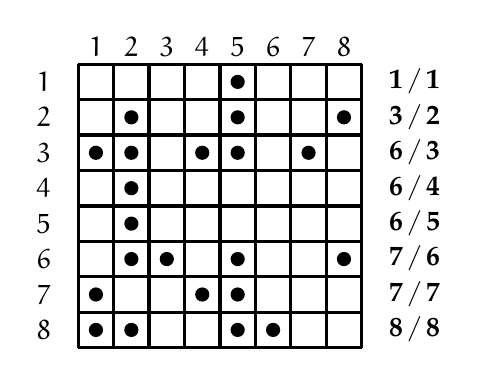
\begin{tikzpicture}[baseline={(current bounding box.center)},scale=0.45]
        \draw[shift={(0.5,0.5)},very thick] (0,0) grid (8,8);
        \foreach \x in {1,2,...,8} {
          \node[left] at (0,9-\x) {$\x$};
        }
        \foreach \y/\x in {1/1,3/2,6/3,6/4,6/5,7/6,7/7,8/8} {
          \node[anchor=west] at (9,9-\x) {$\mathbf{\y\,/\,\x}$};
        }
        \foreach \x in {1,2,...,8} {
          \node at (\x,9) {$\x$};
        }
        \foreach \x/\y in {%
          1/5,
          2/2, 2/5, 2/8,
          3/1, 3/2, 3/4, 3/5, 3/7,
          4/2,
          5/2,
          6/2, 6/3, 6/5, 6/8,
          7/1, 7/4, 7/5,
          8/1, 8/2, 8/5, 8/6} {
            \fill (\y,9-\x) circle(0.2);
        }
      \end{tikzpicture}
      \quad
      \begin{minipage}{.5\textwidth}
        \begin{align*}
          S_1 &= \{x_5\} \\
          S_2 &= \{x_2, x_5, x_8\} \\
          S_3 &= \{x_1, x_2, x_4, x_5, x_7\} \\
          S_4 &= \{x_2\} \\
          S_5 &= \{x_2\} \\
          S_6 &= \{x_2, x_3, x_5, x_8\} \\
          S_7 &= \{x_1, x_4, x_5\} \\
          S_8 &= \{x_1, x_2, x_5, x_6\}
        \end{align*}
    \end{minipage}
    \end{center}
\end{frame}

%%%%%%%%%%%%%%%%%%%%%%%%%%%%%%%%%%%%%%%%%%%%%%%%%%%%%%%%%%%%%%%%%%%%%%%%%%%%%%

\begin{frame}
    \frametitle{Collection of subsets~-~Stepwise bounded labeling}

    \begin{center}
      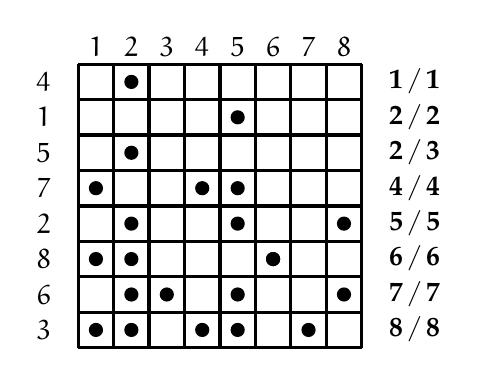
\begin{tikzpicture}[baseline={(current bounding box.center)},scale=0.45]
        \draw[shift={(0.5,0.5)},very thick] (0,0) grid (8,8);
        \foreach \x/\y in {1/4, 2/1, 3/5, 4/7, 5/2, 6/8, 7/6, 8/3} {
          \node[left] at (0,9-\x) {$\y$};
        }
        \foreach \y/\x in {1/1,2/2,2/3,4/4,5/5,6/6,7/7,8/8} {
          \node[anchor=west] at (9,9-\x) {$\mathbf{\y\,/\,\x}$};
        }
        \foreach \x in {1,2,...,8} {
          \node at (\x,9) {$\x$};
        }
        \foreach \x/\y in {%
          1/2,
          2/5,
          3/2,
          4/1, 4/4, 4/5,
          5/2, 5/5, 5/8,
          6/1, 6/2, 6/6, 6/6,
          7/2, 7/3, 7/5, 7/8,
          8/1, 8/2, 8/4, 8/5, 8/7} {
            \fill (\y,9-\x) circle(0.2);
        }
      \end{tikzpicture}
      \quad
      \begin{minipage}{.5\textwidth}
        \begin{align*}
          S_4 &= \{x_2\} \\
          S_1 &= \{x_5\} \\
          S_5 &= \{x_2\} \\
          S_7 &= \{x_1, x_4, x_5\} \\
          S_2 &= \{x_2, x_5, x_8\} \\
          S_8 &= \{x_1, x_2, x_5, x_6\} \\
          S_6 &= \{x_2, x_3, x_5, x_8\} \\
          S_3 &= \{x_1, x_2, x_4, x_5, x_7\}
        \end{align*}
    \end{minipage}
    \end{center}
\end{frame}

%%%%%%%%%%%%%%%%%%%%%%%%%%%%%%%%%%%%%%%%%%%%%%%%%%%%%%%%%%%%%%%%%%%%%%%%%%%%%%

\begin{frame}
    \frametitle{Collection of subsets~-~Stepwise bounded labeling}

    \begin{center}
      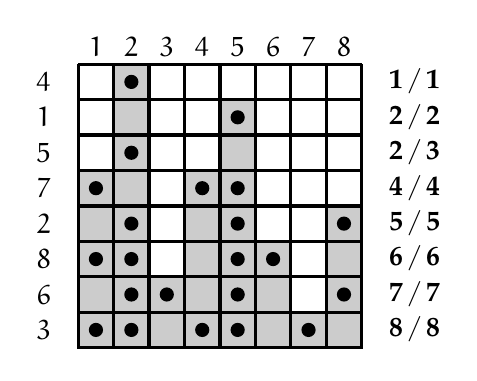
\begin{tikzpicture}[baseline={(current bounding box.center)},scale=0.45]
        \draw [shift={(0.5,0.5)},fill=black!20,very thick]
        (0,0) -- (0,5) -- (1,5) -- (1,8) -- (2,8) --
        (2,2) -- (3,2) -- (3,5) -- (4,5) -- (4,7) --
        (5,7) -- (5,3) -- (6,3) -- (6,1) -- (7,1) --
        (7,4) -- (8,4) -- (8,0) -- cycle;
        \draw[shift={(0.5,0.5)},very thick] (0,0) grid (8,8);
        \foreach \x/\y in {1/4, 2/1, 3/5, 4/7, 5/2, 6/8, 7/6, 8/3} {
          \node[left] at (0,9-\x) {$\y$};
        }
        \foreach \y/\x in {1/1,2/2,2/3,4/4,5/5,6/6,7/7,8/8} {
          \node[anchor=west] at (9,9-\x) {$\mathbf{\y\,/\,\x}$};
        }
        \foreach \x in {1,2,...,8} {
          \node at (\x,9) {$\x$};
        }
        \foreach \x/\y in {%
          1/2,
          2/5,
          3/2,
          4/1, 4/4, 4/5,
          5/2, 5/5, 5/8,
          6/1, 6/2, 6/5, 6/6,
          7/2, 7/3, 7/5, 7/8,
          8/1, 8/2, 8/4, 8/5, 8/7} {
            \fill (\y,9-\x) circle(0.2);
        }
        \end{tikzpicture}
      \quad
      \begin{minipage}{.5\textwidth}
        \begin{align*}
          S_4 &= \{x_2\} \\
          S_1 &= \{x_5\} \\
          S_5 &= \{x_2\} \\
          S_7 &= \{x_1, x_4, x_5\} \\
          S_2 &= \{x_2, x_5, x_8\} \\
          S_8 &= \{x_1, x_2, x_5, x_6\} \\
          S_6 &= \{x_2, x_3, x_5, x_8\} \\
          S_3 &= \{x_1, x_2, x_4, x_5, x_7\}
        \end{align*}
    \end{minipage}
    \end{center}
\end{frame}

%%%%%%%%%%%%%%%%%%%%%%%%%%%%%%%%%%%%%%%%%%%%%%%%%%%%%%%%%%%%%%%%%%%%%%%%%%%%%%

\begin{frame}
    \frametitle{Collection of subsets~-~Permutation-equivalent matrix}

    \begin{center}
      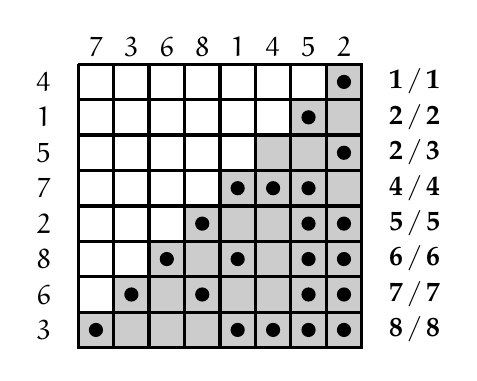
\begin{tikzpicture}[baseline={(current bounding box.center)},scale=0.45]
        \draw [shift={(0.5,0.5)},fill=black!20,very thick]
        (0,0) -- (0,1) -- (1,1) -- (1,2) -- (2,2) --
        (2,3) -- (3,3) -- (3,4) -- (4,4) -- (4,5) --
        (5,5) -- (5,6) -- (6,6) -- (6,7) -- (7,7) --
        (7,8) -- (8,8) -- (8,0) -- cycle;
        \draw[shift={(0.5,0.5)},very thick] (0,0) grid (8,8);
        \foreach \x/\y in {1/4, 2/1, 3/5, 4/7, 5/2, 6/8, 7/6, 8/3} {
          \node[left] at (0,9-\x) {$\y$};
        }
        \foreach \y/\x in {1/1,2/2,2/3,4/4,5/5,6/6,7/7,8/8} {
          \node[anchor=west] at (9,9-\x) {$\mathbf{\y\,/\,\x}$};
        }
        \foreach \x/\y in {1/7, 2/3, 3/6, 4/8, 5/1, 6/4, 7/5, 8/2} {
          \node at (\x,9) {$\y$};
        }
        \foreach \x/\y in {%
          1/8,
          2/7,
          3/8,
          4/5, 4/6, 4/7,
          5/4, 5/7, 5/8,
          6/3, 6/5, 6/7, 6/8,
          7/2, 7/4, 7/7, 7/8,
          8/1, 8/5, 8/6, 8/7, 8/8} {
            \fill (\y,9-\x) circle(0.2);
        }
        \end{tikzpicture}
      \quad
      \begin{minipage}{.5\textwidth}
        \begin{align*}
          S_4 &= \{x_2\} \\
          S_1 &= \{x_5\} \\
          S_5 &= \{x_2\} \\
          S_7 &= \{x_1, x_4, x_5\} \\
          S_2 &= \{x_2, x_5, x_8\} \\
          S_8 &= \{x_1, x_2, x_5, x_6\} \\
          S_6 &= \{x_2, x_3, x_5, x_8\} \\
          S_3 &= \{x_1, x_2, x_4, x_5, x_7\}
        \end{align*}
    \end{minipage}
    \end{center}
\end{frame}

%%%%%%%%%%%%%%%%%%%%%%%%%%%%%%%%%%%%%%%%%%%%%%%%%%%%%%%%%%%%%%%%%%%%%%%%%%%%%%

\begin{frame}
  \frametitle{Collection of subsets}

  \begin{definition}
    Call a bijective mapping
    $\varphi : \mathcal{S} \to [n]$ \textbf{normalized} if $\varphi$
    maps the identical subsets of elements of $\mathcal{S}$
    to a set of consecutive integers.
  \end{definition}


  \bigskip

  Most of the interest in normalized bijective labelings
  stems from the following intuitive lemma.

  \bigskip

  \begin{lemma}
    Let $\mathcal{S} = (S_i : 1 \leq i \leq n)$ be a configuration of subsets of
    some ground $n$-set.
    If there exists a stepwise bounded labeling of $\mathcal{S}$
    then there exists a normalized stepwise bounded labeling of $\mathcal{S}$.
  \end{lemma}
\end{frame}

%%%%%%%%%%%%%%%%%%%%%%%%%%%%%%%%%%%%%%%%%%%%%%%%%%%%%%%%%%%%%%%%%%%%%%%%%%%%%%

\begin{frame}
    \frametitle{Collection of subsets~-~Stepwise bounded labeling}

    \begin{center}
      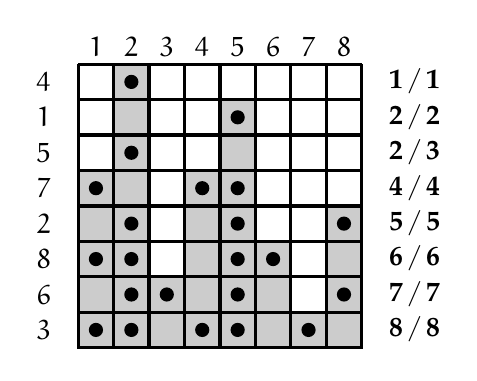
\begin{tikzpicture}[baseline={(current bounding box.center)},scale=0.45]
        \draw [shift={(0.5,0.5)},fill=black!20,very thick]
        (0,0) -- (0,5) -- (1,5) -- (1,8) -- (2,8) --
        (2,2) -- (3,2) -- (3,5) -- (4,5) -- (4,7) --
        (5,7) -- (5,3) -- (6,3) -- (6,1) -- (7,1) --
        (7,4) -- (8,4) -- (8,0) -- cycle;
        \draw[shift={(0.5,0.5)},very thick] (0,0) grid (8,8);
        \foreach \x/\y in {1/4, 2/1, 3/5, 4/7, 5/2, 6/8, 7/6, 8/3} {
          \node[left] at (0,9-\x) {$\y$};
        }
        \foreach \y/\x in {1/1,2/2,2/3,4/4,5/5,6/6,7/7,8/8} {
          \node[anchor=west] at (9,9-\x) {$\mathbf{\y\,/\,\x}$};
        }
        \foreach \x in {1,2,...,8} {
          \node at (\x,9) {$\x$};
        }
        \foreach \x/\y in {%
          1/2,
          2/5,
          3/2,
          4/1, 4/4, 4/5,
          5/2, 5/5, 5/8,
          6/1, 6/2, 6/5, 6/6,
          7/2, 7/3, 7/5, 7/8,
          8/1, 8/2, 8/4, 8/5, 8/7} {
            \fill (\y,9-\x) circle(0.2);
        }
        \end{tikzpicture}
      \quad
      \begin{minipage}{.5\textwidth}
        \begin{align*}
          S_4 &= \{x_2\} \\
          S_1 &= \{x_5\} \\
          S_5 &= \{x_2\} \\
          S_7 &= \{x_1, x_4, x_5\} \\
          S_2 &= \{x_2, x_5, x_8\} \\
          S_8 &= \{x_1, x_2, x_5, x_6\} \\
          S_6 &= \{x_2, x_3, x_5, x_8\} \\
          S_3 &= \{x_1, x_2, x_4, x_5, x_7\}
        \end{align*}
    \end{minipage}
    \end{center}
\end{frame}

%%%%%%%%%%%%%%%%%%%%%%%%%%%%%%%%%%%%%%%%%%%%%%%%%%%%%%%%%%%%%%%%%%%%%%%%%%%%%%

\begin{frame}
    \frametitle{Collection of subsets~-~Normalized stepwise bounded labeling}

    \begin{center}
      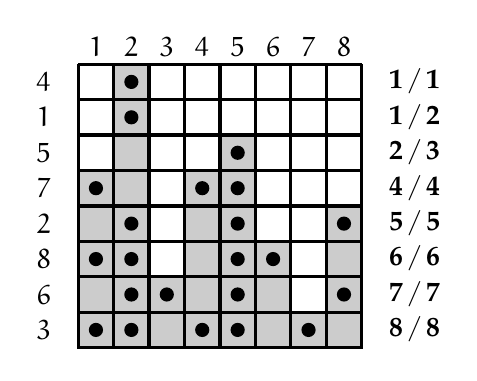
\begin{tikzpicture}[baseline={(current bounding box.center)},scale=0.45]
        \draw [shift={(0.5,0.5)},fill=black!20,very thick]
        (0,0) -- (0,5) -- (1,5) -- (1,8) -- (2,8) --
        (2,2) -- (3,2) -- (3,5) -- (4,5) -- (4,6) --
        (5,6) -- (5,3) -- (6,3) -- (6,1) -- (7,1) --
        (7,4) -- (8,4) -- (8,0) -- cycle;
        \draw[shift={(0.5,0.5)},very thick] (0,0) grid (8,8);
        \foreach \x/\y in {1/4, 2/1, 3/5, 4/7, 5/2, 6/8, 7/6, 8/3} {
          \node[left] at (0,9-\x) {$\y$};
        }
        \foreach \y/\x in {1/1,1/2,2/3,4/4,5/5,6/6,7/7,8/8} {
          \node[anchor=west] at (9,9-\x) {$\mathbf{\y\,/\,\x}$};
        }
        \foreach \x in {1,2,...,8} {
          \node at (\x,9) {$\x$};
        }
        \foreach \x/\y in {%
          1/2,
          2/2,
          3/5,
          4/1, 4/4, 4/5,
          5/2, 5/5, 5/8,
          6/1, 6/2, 6/5, 6/6,
          7/2, 7/3, 7/5, 7/8,
          8/1, 8/2, 8/4, 8/5, 8/7} {
            \fill (\y,9-\x) circle(0.2);
        }
        \end{tikzpicture}
      \quad
      \begin{minipage}{.5\textwidth}
        \begin{align*}
          S_4 &= \{x_2\} \\
          S_5 &= \{x_2\} \\
          S_1 &= \{x_5\} \\
          S_7 &= \{x_1, x_4, x_5\} \\
          S_2 &= \{x_2, x_5, x_8\} \\
          S_8 &= \{x_1, x_2, x_5, x_6\} \\
          S_6 &= \{x_2, x_3, x_5, x_8\} \\
          S_3 &= \{x_1, x_2, x_4, x_5, x_7\}
        \end{align*}
    \end{minipage}
    \end{center}
\end{frame}

%%%%%%%%%%%%%%%%%%%%%%%%%%%%%%%%%%%%%%%%%%%%%%%%%%%%%%%%%%%%%%%%%%%%%%%%%%%%%%

\begin{frame}
    \frametitle{Main result}

    \begin{theorem}
      Let $\mathcal{S} = (S_i : 1 \leq i \leq n)$ be a configuration of subsets of
      some ground $n$-set.
      Deciding whether there exists a stepwise bounded labeling of $\mathcal{S}$
      is \NPC.
    \end{theorem}

    \bigskip

    \begin{itemize}
      \item
      The proof proceeds by a reduction from the \NPcomplete \PB{3Sat} problem.

      \item
      Focus on normalized stepwise bounded labelings.
    \end{itemize}

\end{frame}

%%%%%%%%%%%%%%%%%%%%%%%%%%%%%%%%%%%%%%%%%%%%%%%%%%%%%%%%%%%%%%%%%%%%%%%%%%%%%%

\begin{frame}
    \frametitle{Reduction: Big picture}

    \begin{center}
      \includegraphics[scale=.7]{reduction.pdf}
    \end{center}

\end{frame}

%%%%%%%%%%%%%%%%%%%%%%%%%%%%%%%%%%%%%%%%%%%%%%%%%%%%%%%%%%%%%%%%%%%%%%%%%%%%%%

\begin{frame}
    \frametitle{Reduction: Big picture -- Literal selection}

    \begin{center}
      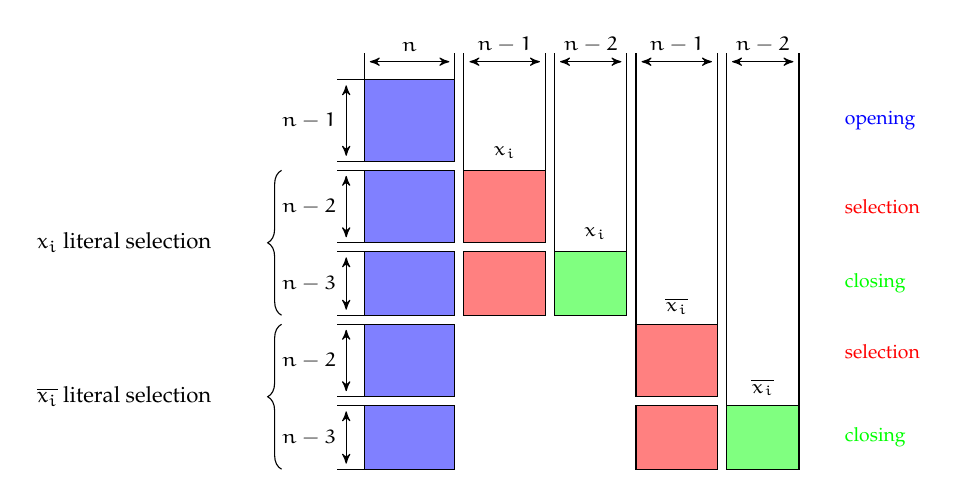
\begin{tikzpicture}[scale=0.115]
        \onslide<1->
        %
        \draw [fill=blue!50] (0,0) rectangle (10,9);
        \draw (52,4.5) node [anchor=west] {\scriptsize \textcolor{blue}{opening}};
        %
        \draw (-3,9) -- (0,9);
        \draw (-3,0) -- (0,0);
        \draw [shorten >=2pt,shorten <=2pt,>=stealth',arrows=<->]
        (-2,0) -- node [left] {\scriptsize $n-1$} ++ (0,9);
        %
        \draw (0,9) -- (0,12);
        \draw (10,9) -- (10,12);
        \draw [shorten >=2pt,shorten <=2pt,>=stealth',arrows=<->]
        (0,11) -- node [above] {\scriptsize $n$} ++ (10,0);
        %
        \onslide<2->
        %
        \draw [fill=blue!50] (0,-9) rectangle (10,-1);
        \draw [fill=red!50] (11,-9) rectangle (20,-1);
        \draw (15.5, 1) node []
        {\scriptsize $x_i$};
        \draw (52,-5) node [anchor=west] {\scriptsize \textcolor{red}{selection}};
        %
        \draw [fill=blue!50] (0,-17) rectangle (10,-10);
        \draw [fill=red!50] (11,-17) rectangle (20,-10);
        \draw [fill=green!50] (21,-17) rectangle (29,-10);
        \draw (25.5, -8) node []
        {\scriptsize $x_i$};
        \draw (52,-13.5) node [anchor=west] {\scriptsize \textcolor{green}{closing}};
        %
        \draw (-3,-1) -- (0,-1);
        \draw (-3,-9) -- (0,-9);
        \draw [shorten >=2pt,shorten <=2pt,>=stealth',arrows=<->]
        (-2,-9) -- node [left] {\scriptsize $n-2$} ++ (0,8);
        %
        \draw (-3,-17) -- (0,-17);
        \draw (-3,-10) -- (0,-10);
        \draw [shorten >=2pt,shorten <=2pt,>=stealth',arrows=<->]
        (-2,-17) -- node [left] {\scriptsize $n-3$} ++ (0,7);
        %
        \draw [decorate,decoration={brace,amplitude=5pt},xshift=-4pt,yshift=0pt]
        (-9,-17) -- (-9,-1) node [black,midway,xshift=-2cm]
        {\footnotesize $x_i$ literal selection};
        %
        \draw (11,-1) -- (11,12);
        \draw (20,-1) -- (20,12);
        \draw [shorten >=2pt,shorten <=2pt,>=stealth',arrows=<->]
        (11,11) -- node [above] {\scriptsize $n-1$} ++ (9,0);
        %
        \draw (21,-17) -- (21,12);
        \draw (29,-17) -- (29,12);
        \draw [shorten >=2pt,shorten <=2pt,>=stealth',arrows=<->]
        (21,11) -- node [above] {\scriptsize $n-2$} ++ (8,0);
        %
        \onslide<3->
        %
        \draw [fill=blue!50] (0,-26) rectangle (10,-18);
        \draw [fill=red!50] (30,-26) rectangle (39,-18);
        \draw (34.5, -16) node []
        {\scriptsize $\overline{x_i}$};
        \draw (52,-21) node [anchor=west] {\scriptsize \textcolor{red}{selection}};
        %
        \draw [fill=blue!50] (0,-34) rectangle (10,-27);
        \draw [fill=red!50] (30,-34) rectangle (39,-27);
        \draw [fill=green!50] (40,-34) rectangle (48,-27);
        \draw (44, -25) node []
        {\scriptsize $\overline{x_i}$};
        %
        \draw (52,-30.5) node [anchor=west] {\scriptsize \textcolor{green}{closing}};
        %
        \draw (-3,-18) -- (0,-18);
        \draw (-3,-26) -- (0,-26);
        \draw [shorten >=2pt,shorten <=2pt,>=stealth',arrows=<->]
        (-2,-26) -- node [left] {\scriptsize $n-2$} ++ (0,8);
        %
        \draw (-3,-27) -- (0,-27);
        \draw (-3,-34) -- (0,-34);
        \draw [shorten >=2pt,shorten <=2pt,>=stealth',arrows=<->]
        (-2,-34) -- node [left] {\scriptsize $n-3$} ++ (0,7);
        %
        \draw [decorate,decoration={brace,amplitude=5pt},xshift=-4pt,yshift=0pt]
        (-9,-34) -- (-9,-18) node [black,midway,xshift=-2cm]
        {\footnotesize $\overline{x_{i}}$ literal selection};
        %
        \draw (30,-18) -- (30,12);
        \draw (39,-18) -- (39,12);
        \draw [shorten >=2pt,shorten <=2pt,>=stealth',arrows=<->]
        (30,11) -- node [above] {\scriptsize $n-1$} ++ (9,0);
        %
        \draw (40,-27) -- (40,12);
        \draw (48,-27) -- (48,12);
        \draw [shorten >=2pt,shorten <=2pt,>=stealth',arrows=<->]
        (40,11) -- node [above] {\scriptsize $n-2$} ++ (8,0);
      \end{tikzpicture}
    \end{center}

\end{frame}

%%%%%%%%%%%%%%%%%%%%%%%%%%%%%%%%%%%%%%%%%%%%%%%%%%%%%%%%%%%%%%%%%%%%%%%%%%%%%%

\begin{frame}
    \frametitle{Reduction: Big picture -- Literal selection}

    \begin{center}
      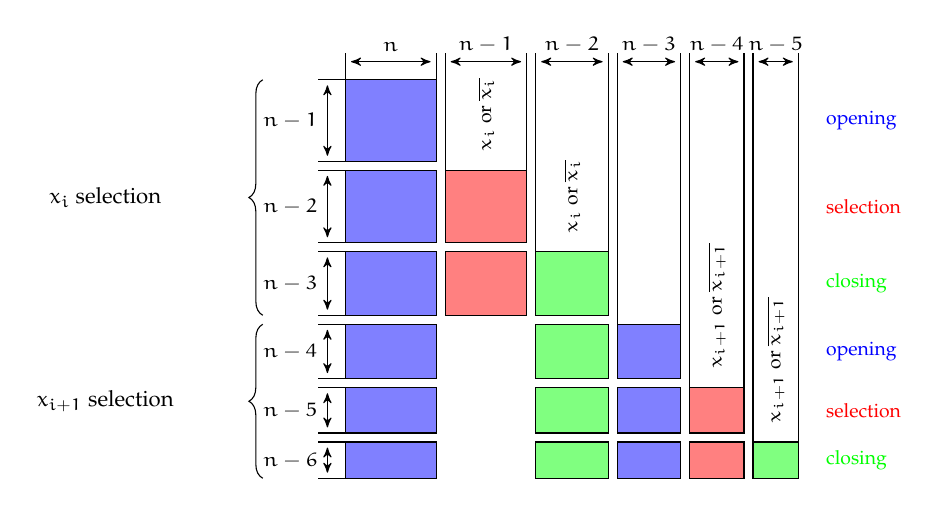
\begin{tikzpicture}[scale=0.115]
        \onslide<1->
        %
        \draw [fill=blue!50] (0,0) rectangle (10,9);
        \draw (52,4.5) node [anchor=west] {\scriptsize \textcolor{blue}{opening}};
        %
        \draw [fill=blue!50] (0,-9) rectangle (10,-1);
        \draw [fill=red!50] (11,-9) rectangle (20,-1);
        \draw (15.5, 0) node [anchor=west,rotate=90]
        {\scriptsize $x_i$ or $\overline{x_i}$};
        \draw (52,-5) node [anchor=west] {\scriptsize \textcolor{red}{selection}};
        %
        \draw [fill=blue!50] (0,-17) rectangle (10,-10);
        \draw [fill=red!50] (11,-17) rectangle (20,-10);
        \draw [fill=green!50] (21,-17) rectangle (29,-10);
        \draw (25, -9) node [anchor=west,rotate=90]
        {\scriptsize $x_i$ or $\overline{x_i}$};
        \draw (52,-13.5) node [anchor=west] {\scriptsize \textcolor{green}{closing}};
        %
        \draw (-3,9) -- (0,9);
        \draw (-3,0) -- (0,0);
        \draw [shorten >=2pt,shorten <=2pt,>=stealth',arrows=<->]
        (-2,0) -- node [left] {\scriptsize $n-1$} ++ (0,9);
        %
        \draw (-3,-1) -- (0,-1);
        \draw (-3,-9) -- (0,-9);
        \draw [shorten >=2pt,shorten <=2pt,>=stealth',arrows=<->]
        (-2,-9) -- node [left] {\scriptsize $n-2$} ++ (0,8);
        %
        \draw (-3,-17) -- (0,-17);
        \draw (-3,-10) -- (0,-10);
        \draw [shorten >=2pt,shorten <=2pt,>=stealth',arrows=<->]
        (-2,-17) -- node [left] {\scriptsize $n-3$} ++ (0,7);
        %
        \draw [decorate,decoration={brace,amplitude=5pt},xshift=-4pt,yshift=0pt]
        (-9,-17) -- (-9,9) node [black,midway,xshift=-2cm]
        {\footnotesize $x_i$ selection};
        %
        \draw (0,9) -- (0,12);
        \draw (10,9) -- (10,12);
        \draw [shorten >=2pt,shorten <=2pt,>=stealth',arrows=<->]
        (0,11) -- node [above] {\scriptsize $n$} ++ (10,0);
        %
        \draw (11,-1) -- (11,12);
        \draw (20,-1) -- (20,12);
        \draw [shorten >=2pt,shorten <=2pt,>=stealth',arrows=<->]
        (11,11) -- node [above] {\scriptsize $n-1$} ++ (9,0);
        %
        \draw (21,-17) -- (21,12);
        \draw (29,-17) -- (29,12);
        \draw [shorten >=2pt,shorten <=2pt,>=stealth',arrows=<->]
        (21,11) -- node [above] {\scriptsize $n-2$} ++ (8,0);
        %
        \onslide<2>
        %
        %
        \draw [fill=blue!50] (0,-24) rectangle (10,-18);
        \draw [fill=green!50] (21,-24) rectangle (29,-18);
        \draw [fill=blue!50] (30,-24) rectangle (37,-18);
        \draw (52,-21) node [anchor=west] {\scriptsize \textcolor{blue}{opening}};
        %
        \draw [fill=blue!50] (0,-30) rectangle (10,-25);
        \draw [fill=green!50] (21,-30) rectangle (29,-25);
        \draw [fill=blue!50] (30,-30) rectangle (37,-25);
        \draw [fill=red!50] (38,-30) rectangle (44,-25);
        \draw (41, -24) node [anchor=west,rotate=90]
        {\scriptsize $x_{i+1}$ or $\overline{x_{i+1}}$};
        \draw (52,-27.5) node [anchor=west] {\scriptsize \textcolor{red}{selection}};
        %
        \draw [fill=blue!50] (0,-35) rectangle (10,-31);
        \draw [fill=green!50] (21,-35) rectangle (29,-31);
        \draw [fill=blue!50] (30,-35) rectangle (37,-31);
        \draw [fill=red!50] (38,-35) rectangle (44,-31);
        \draw [fill=green!50] (45,-35) rectangle (50,-31);
        \draw (47.5, -30) node [anchor=west,rotate=90]
        {\scriptsize $x_{i+1}$ or $\overline{x_{i+1}}$};
        \draw (52,-33) node [anchor=west] {\scriptsize \textcolor{green}{closing}};
        %
        \draw (-3,-18) -- (0,-18);
        \draw (-3,-24) -- (0,-24);
        \draw [shorten >=2pt,shorten <=2pt,>=stealth',arrows=<->]
        (-2,-24) -- node [left] {\scriptsize $n-4$} ++ (0,6);
        %
        \draw (-3,-30) -- (0,-30);
        \draw (-3,-25) -- (0,-25);
        \draw [shorten >=2pt,shorten <=2pt,>=stealth',arrows=<->]
        (-2,-30) -- node [left] {\scriptsize $n-5$} ++ (0,5);
        %
        \draw (-3,-31) -- (0,-31);
        \draw (-3,-35) -- (0,-35);
        \draw [shorten >=2pt,shorten <=2pt,>=stealth',arrows=<->]
        (-2,-35) -- node [left] {\scriptsize $n-6$} ++ (0,4);
        %
        \draw [decorate,decoration={brace,amplitude=5pt},xshift=-4pt,yshift=0pt]
        (-9,-35) -- (-9,-18) node [black,midway,xshift=-2cm]
        {\footnotesize $x_{i+1}$ selection};
        %
        \draw (30,-18) -- (30,12);
        \draw (37,-18) -- (37,12);
        \draw [shorten >=2pt,shorten <=2pt,>=stealth',arrows=<->]
        (30,11) -- node [above] {\scriptsize $n-3$} ++ (7,0);
        %
        \draw (38,-25) -- (38,12);
        \draw (44,-30) -- (44,12);
        \draw [shorten >=2pt,shorten <=2pt,>=stealth',arrows=<->]
        (38,11) -- node [above] {\scriptsize $n-4$} ++ (6,0);
        %
        \draw (45,-31) -- (45,12);
        \draw (50,-31) -- (50,12);
        \draw [shorten >=2pt,shorten <=2pt,>=stealth',arrows=<->]
        (45,11) -- node [above] {\scriptsize $n-5$} ++ (5,0);

      \end{tikzpicture}
    \end{center}

\end{frame}

%%%%%%%%%%%%%%%%%%%%%%%%%%%%%%%%%%%%%%%%%%%%%%%%%%%%%%%%%%%%%%%%%%%%%%%%%%%%%%

\begin{frame}
    \frametitle{Reduction: Big picture -- Literal in clause selection}

    \begin{center}
      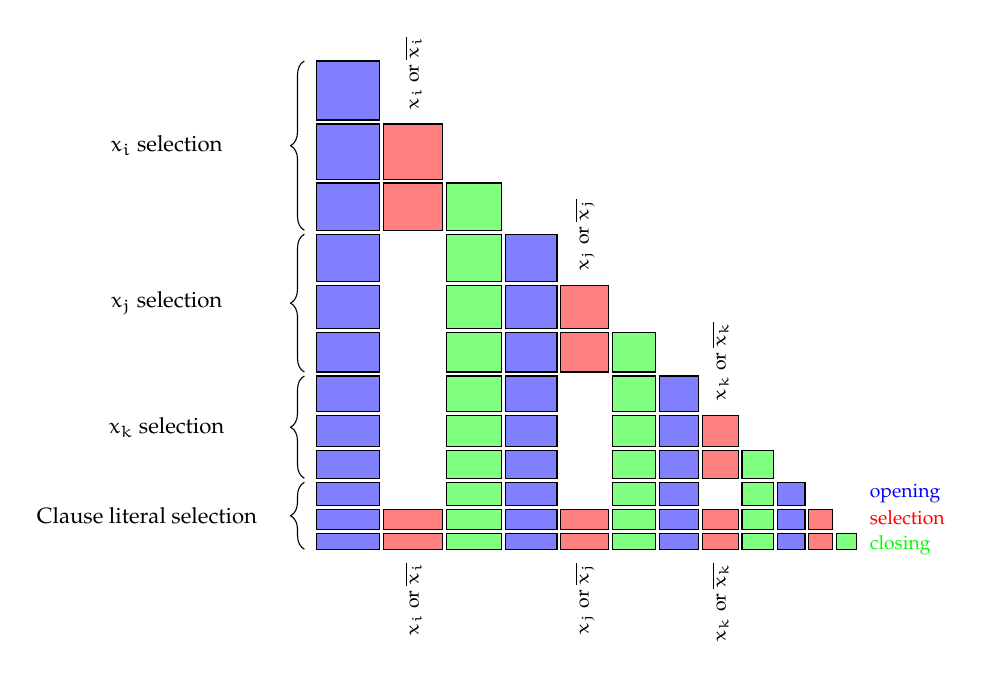
\begin{tikzpicture}[scale=0.05]
        \onslide<1->
        \draw [fill=blue!50] (0,18) rectangle (16,25);
        \draw [fill=green!50] (33,18) rectangle (47,25);
        \draw [fill=blue!50] (48,18) rectangle (61,25);
        \draw [fill=green!50] (75,18) rectangle (86,25);
        \draw [fill=blue!50] (87,18) rectangle (97,25);
        \draw [fill=red!50] (98,18) rectangle (107,25);
        \draw [fill=green!50] (108,18) rectangle (116,25);
        %
        \draw [fill=blue!50] (0,26) rectangle (16,34);
        \draw [fill=green!50] (33,26) rectangle (47,34);
        \draw [fill=blue!50] (48,26) rectangle (61,34);
        \draw [fill=green!50] (75,26) rectangle (86,34);
        \draw [fill=blue!50] (87,26) rectangle (97,34);
        \draw [fill=red!50] (98,26) rectangle (107,34);
        \draw (102.5, 35) node [anchor=west,rotate=90]
        {\scriptsize $x_k$ or $\overline{x_k}$};
        %
        \draw [decorate,decoration={brace,amplitude=5pt},xshift=-4pt,yshift=0pt]
        (-3,18) -- (-3,44) node [black,midway,xshift=-1.75cm]
        {\footnotesize $x_k$ selection};
        %
        \draw [fill=blue!50] (0,35) rectangle (16,44);
        \draw [fill=green!50] (33,35) rectangle (47,44);
        \draw [fill=blue!50] (48,35) rectangle (61,44);
        \draw [fill=green!50] (75,35) rectangle (86,44);
        \draw [fill=blue!50] (87,35) rectangle (97,44);
        %
        \draw [fill=blue!50] (0,45) rectangle (16,55);
        \draw [fill=green!50] (33,45) rectangle (47,55);
        \draw [fill=blue!50] (48,45) rectangle (61,55);
        \draw [fill=red!50] (62,45) rectangle (74,55);
        \draw [fill=green!50] (75,45) rectangle (86,55);
        %
        \draw [fill=blue!50] (0,56) rectangle (16,67);
        \draw [fill=green!50] (33,56) rectangle (47,67);
        \draw [fill=blue!50] (48,56) rectangle (61,67);
        \draw [fill=red!50] (62,56) rectangle (74,67);
        \draw (68, 68) node [anchor=west,rotate=90]
        {\scriptsize $x_j$ or $\overline{x_j}$};
        %
        \draw [decorate,decoration={brace,amplitude=5pt},xshift=-4pt,yshift=0pt]
        (-3,45) -- (-3,80) node [black,midway,xshift=-1.75cm]
        {\footnotesize $x_j$ selection};
        %
        \draw [fill=blue!50] (0,68) rectangle (16,80);
        \draw [fill=green!50] (33,68) rectangle (47,80);
        \draw [fill=blue!50] (48,68) rectangle (61,80);
        %
        \draw [fill=blue!50] (0,81) rectangle (16,93);
        \draw [fill=red!50] (17,81) rectangle (32,93);
        \draw [fill=green!50] (33,81) rectangle (47,93);
        %
        \draw [fill=blue!50] (0,94) rectangle (16,108);
        \draw [fill=red!50] (17,94) rectangle (32,108);
        \draw (24.5, 109) node [anchor=west,rotate=90]
        {\scriptsize $x_i$ or $\overline{x_i}$};
        %
        \draw [fill=blue!50] (0,109) rectangle (16,124);
        %
        \draw [decorate,decoration={brace,amplitude=5pt},xshift=-4pt,yshift=0pt]
        (-3,81) -- (-3,124) node [black,midway,xshift=-1.75cm]
        {\footnotesize $x_i$ selection};
        %
        \onslide<2->
        %
        \draw [fill=blue!50] (0,11) rectangle (16,17);
        \draw [fill=green!50] (33,11) rectangle (47,17);
        \draw [fill=blue!50] (48,11) rectangle (61,17);
        \draw [fill=green!50] (75,11) rectangle (86,17);
        \draw [fill=blue!50] (87,11) rectangle (97,17);
        \draw [fill=green!50] (108,11) rectangle (116,17);
        \draw [fill=blue!50] (117,11) rectangle (124,17);
        \draw (138,14) node [anchor=west]
        {\scriptsize \textcolor{blue}{opening}};
        %
        \draw [fill=blue!50] (0,5) rectangle (16,10);
        \draw [fill=green!50] (33,5) rectangle (47,10);
        \draw [fill=blue!50] (48,5) rectangle (61,10);
        \draw [fill=green!50] (75,5) rectangle (86,10);
        \draw [fill=blue!50] (87,5) rectangle (97,10);
        \draw [fill=green!50] (108,5) rectangle (116,10);
        \draw [fill=blue!50] (117,5) rectangle (124,10);
        \draw [fill=red!50] (125,5) rectangle (131,10);
        \draw (138,8) node [anchor=west]
        {\scriptsize \textcolor{red}{selection}};
        %
        \draw [fill=blue!50] (0,0) rectangle (16,4);
        \draw [fill=green!50] (33,0) rectangle (47,4);
        \draw [fill=blue!50] (48,0) rectangle (61,4);
        \draw [fill=green!50] (75,0) rectangle (86,4);
        \draw [fill=blue!50] (87,0) rectangle (97,4);
        \draw [fill=green!50] (108,0) rectangle (116,4);
        \draw [fill=blue!50] (117,0) rectangle (124,4);
        \draw [fill=red!50] (125,0) rectangle (131,4);
        \draw [fill=green!50] (132,0) rectangle (137,4);
        \draw (138,1) node [anchor=west]
        {\scriptsize \textcolor{green}{closing}};
        %
        \draw [decorate,decoration={brace,amplitude=5pt},xshift=-4pt,yshift=0pt]
        (-3,0) -- (-3,17) node [black,midway,xshift=-2cm]
        {\footnotesize Clause literal selection};
        %
        \onslide<3>
        \draw [fill=red!50] (17,5) rectangle (32,10);
        \draw [fill=red!50] (17,0) rectangle (32,4);
        \draw (24.5, -1) node [anchor=east,rotate=90]
        {\scriptsize $x_i$ or $\overline{x_i}$};
        %
        \onslide<4>
        \draw [fill=red!50] (62,5) rectangle (74,10);
        \draw [fill=red!50] (62,0) rectangle (74,4);
        \draw (68, -1) node [anchor=east,rotate=90]
        {\scriptsize $x_j$ or $\overline{x_j}$};
        %
        \onslide<5>
        \draw [fill=red!50] (98,5) rectangle (107,10);
        \draw [fill=red!50] (98,0) rectangle (107,4);
        \draw (102.5, -1) node [anchor=east,rotate=90]
        {\scriptsize $x_k$ or $\overline{x_k}$};
      \end{tikzpicture}
    \end{center}

\end{frame}

%%%%%%%%%%%%%%%%%%%%%%%%%%%%%%%%%%%%%%%%%%%%%%%%%%%%%%%%%%%%%%%%%%%%%%%%%%%%%%

%%%%%%%%%%%%%%%%%%%%%%%%%%%%%%%%%%%%%%%%%%%%%%%%%%%%%%%%%%%%%%%%%%%%%%%%%%%%%%

\begin{frame}
  \frametitle{Solving the problem (exponential-time algorithm)}

  \begin{itemize}
    \item
    Simple divide-and-conquer algorithm.

    \bigskip

    \item
    "\emph{If a matrix is permutation equivalent to a triangular matrix then
    it contains a large $0$ square submatrix}"

    \bigskip

    \item
    Still pretty slow in practice
    (more effort should be directed towards
    improving the running-time of the program!)
  \end{itemize}
\end{frame}

%%%%%%%%%%%%%%%%%%%%%%%%%%%%%%%%%%%%%%%%%%%%%%%%%%%%%%%%%%%%%%%%%%%%%%%%%%%%%%

\begin{frame}
  \frametitle{Algorithm -- Main idea}

  \bigskip

  \begin{overprint}
    \onslide<1>
    \begin{center}
      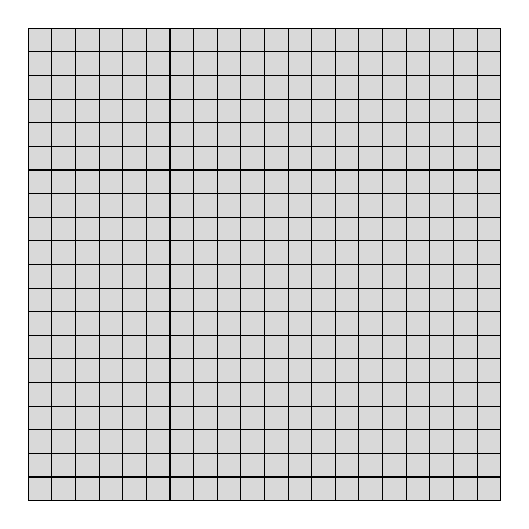
\begin{tikzpicture}[scale=0.3]
        \draw [fill=black!15] (0,0) rectangle (20,20);
        \draw [] (0,0) grid (20,20);
      \end{tikzpicture}
    \end{center}

    Initial configuration.

    \onslide<2>
    \begin{center}
      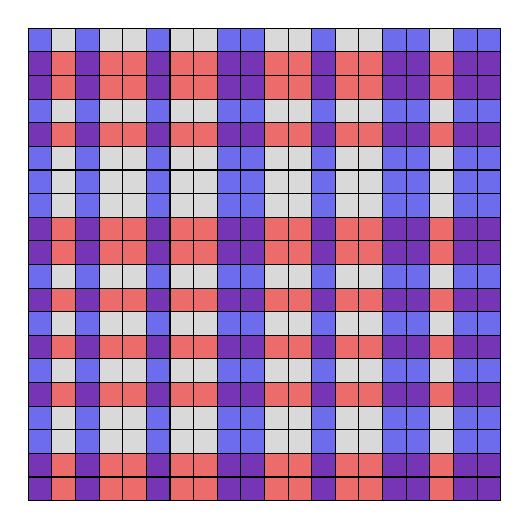
\begin{tikzpicture}[scale=0.3]
        \draw [fill=black!15] (0,0) rectangle (20,20);
        %
        \draw [fill=red, opacity=0.5] (0,18) rectangle (20,19);
        \draw [fill=red, opacity=0.5] (0,17) rectangle (20,18);
        \draw [fill=red, opacity=0.5] (0,15) rectangle (20,16);
        \draw [fill=red, opacity=0.5] (0,11) rectangle (20,12);
        \draw [fill=red, opacity=0.5] (0,10) rectangle (20,11);
        \draw [fill=red, opacity=0.5] (0,8) rectangle (20,9);
        \draw [fill=red, opacity=0.5] (0,6) rectangle (20,7);
        \draw [fill=red, opacity=0.5] (0,4) rectangle (20,5);
        \draw [fill=red, opacity=0.5] (0,1) rectangle (20,2);
        \draw [fill=red, opacity=0.5] (0,0) rectangle (20,1);
        %
        \draw [fill=blue, opacity=0.5] (0,0) rectangle (1,20);
        \draw [fill=blue, opacity=0.5] (2,0) rectangle (3,20);
        \draw [fill=blue, opacity=0.5] (5,0) rectangle (6,20);
        \draw [fill=blue, opacity=0.5] (8,0) rectangle (9,20);
        \draw [fill=blue, opacity=0.5] (9,0) rectangle (10,20);
        \draw [fill=blue, opacity=0.5] (12,0) rectangle (13,20);
        \draw [fill=blue, opacity=0.5] (15,0) rectangle (16,20);
        \draw [fill=blue, opacity=0.5] (16,0) rectangle (17,20);
        \draw [fill=blue, opacity=0.5] (18,0) rectangle (19,20);
        \draw [fill=blue, opacity=0.5] (19,0) rectangle (20,20);
        %
        \draw [] (0,0) grid (20,20);
      \end{tikzpicture}
    \end{center}

    Guess \textcolor{red}{$n/2$ rows} and \textcolor{blue}{$n/2$ columns}.

    \onslide<3>
    \begin{center}
      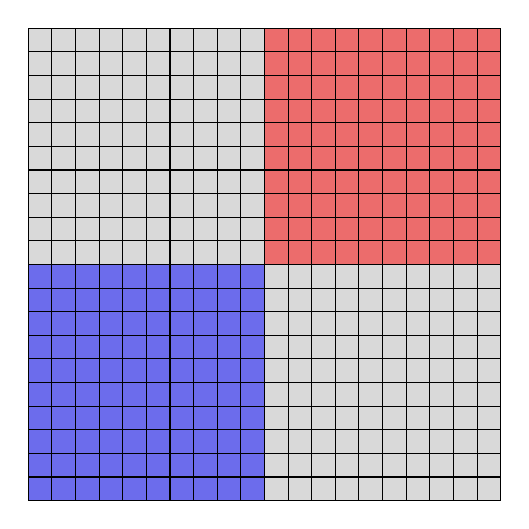
\begin{tikzpicture}[scale=0.3]
        \draw [fill=black!15] (0,0) rectangle (20,20);
        %
        \draw [fill=red, opacity=0.5] (10,10) rectangle (20,20);
        %
        \draw [fill=blue, opacity=0.5] (0,0) rectangle (10,10);
        %
        \draw [] (0,0) grid (20,20);
      \end{tikzpicture}
    \end{center}

    Permute rows and columns according to the selected rows and columns.

    \onslide<4>
    \begin{center}
      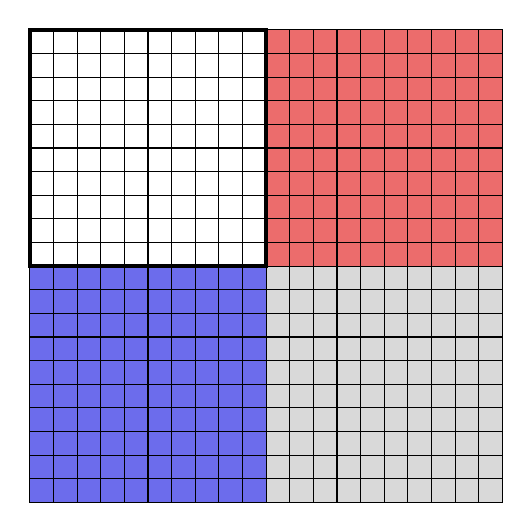
\begin{tikzpicture}[scale=0.3]
        \draw [fill=black!15] (0,0) rectangle (10,10);
        \draw [fill=black!15] (10,0) rectangle (20,10);
        \draw [fill=black!15] (10,10) rectangle (20,20);
        %
        \draw [fill=red, opacity=0.5] (10,10) rectangle (20,20);
        %
        \draw [fill=blue, opacity=0.5] (0,0) rectangle (10,10);
        %
        \draw [ultra thick] (0,10) rectangle (10,20);
        %
        \draw [] (0,0) grid (20,20);
      \end{tikzpicture}
    \end{center}

    Check top left submatrix is $0$.

    \onslide<5>
    \begin{center}
      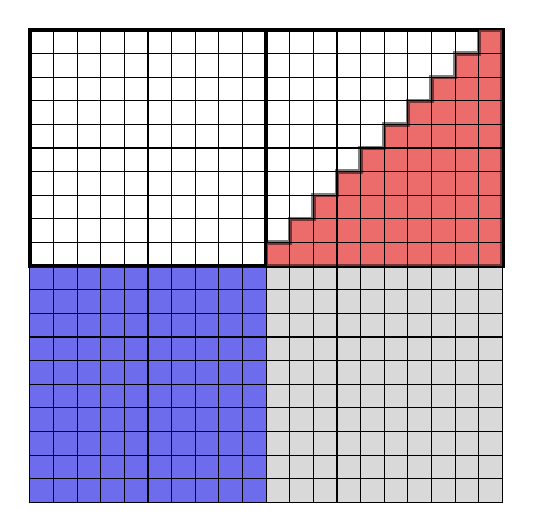
\begin{tikzpicture}[scale=0.3]
        \draw [fill=black!15] (0,0) rectangle (10,10);
        \draw [fill=black!15] (10,0) rectangle (20,10);
        %
        \draw [ultra thick] (0,10) rectangle (10,20);
        \draw [ultra thick] (10,10) rectangle (20,20);
        %
        \draw [fill=blue, opacity=0.5] (0,0) rectangle (10,10);
        %
        \draw [fill=black!15]
        (10,10) -- (10,11) -- (11,11) -- (11,12) -- (12,12) --
        (12,13) -- (13,13) -- (13,14) -- (14,14) -- (14,15) --
        (15,15) -- (15,16) -- (16,16) -- (16,17) -- (17,17) --
        (17,18) -- (18,18) -- (18,19) -- (19,19) -- (19,20) --
        (20,20) -- (20,10) -- cycle;
        \draw [ultra thick,fill=red, opacity=0.5]
        (10,10) -- (10,11) -- (11,11) -- (11,12) -- (12,12) --
        (12,13) -- (13,13) -- (13,14) -- (14,14) -- (14,15) --
        (15,15) -- (15,16) -- (16,16) -- (16,17) -- (17,17) --
        (17,18) -- (18,18) -- (18,19) -- (19,19) -- (19,20) --
        (20,20) -- (20,10) -- cycle;
        %
        \draw [] (0,0) grid (20,20);
      \end{tikzpicture}
    \end{center}

    Recurse on top right submatrix.

    \onslide<6>
    \begin{center}
      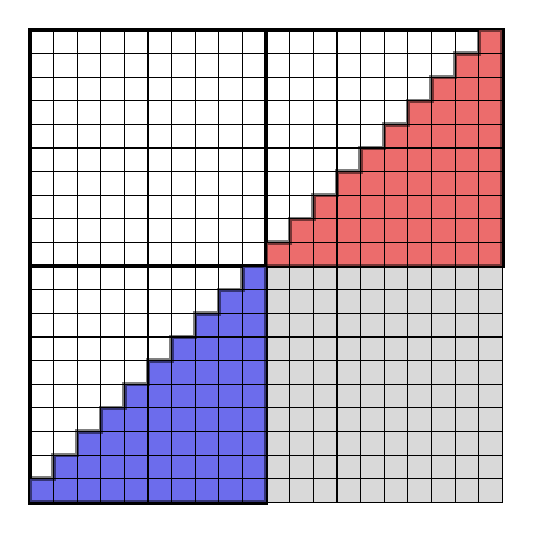
\begin{tikzpicture}[scale=0.3]
        \draw [fill=black!15] (10,0) rectangle (20,10);
        %
        \draw [ultra thick] (0,10) rectangle (10,20);
        \draw [ultra thick] (10,10) rectangle (20,20);
        \draw [ultra thick] (0,0) rectangle (10,10);
        %
        \draw [fill=black!15]
        (10,10) -- (10,11) -- (11,11) -- (11,12) -- (12,12) --
        (12,13) -- (13,13) -- (13,14) -- (14,14) -- (14,15) --
        (15,15) -- (15,16) -- (16,16) -- (16,17) -- (17,17) --
        (17,18) -- (18,18) -- (18,19) -- (19,19) -- (19,20) --
        (20,20) -- (20,10) -- cycle;
        \draw [ultra thick,fill=red, opacity=0.5]
        (10,10) -- (10,11) -- (11,11) -- (11,12) -- (12,12) --
        (12,13) -- (13,13) -- (13,14) -- (14,14) -- (14,15) --
        (15,15) -- (15,16) -- (16,16) -- (16,17) -- (17,17) --
        (17,18) -- (18,18) -- (18,19) -- (19,19) -- (19,20) --
        (20,20) -- (20,10) -- cycle;
        \draw [fill=black!15]
        (0,0) -- (0,1) -- (1,1) -- (1,2) -- (2,2) --
        (2,3) -- (3,3) -- (3,4) -- (4,4) -- (4,5) --
        (5,5) -- (5,6) -- (6,6) -- (6,7) -- (7,7) --
        (7,8) -- (8,8) -- (8,9) -- (9,9) -- (9,10) --
        (10,10) -- (10,0) -- cycle;
        \draw [ultra thick,fill=blue, opacity=0.5]
        (0,0) -- (0,1) -- (1,1) -- (1,2) -- (2,2) --
        (2,3) -- (3,3) -- (3,4) -- (4,4) -- (4,5) --
        (5,5) -- (5,6) -- (6,6) -- (6,7) -- (7,7) --
        (7,8) -- (8,8) -- (8,9) -- (9,9) -- (9,10) --
        (10,10) -- (10,0) -- cycle;
        %
        \draw [] (0,0) grid (20,20);
      \end{tikzpicture}
    \end{center}

    Recurse on bottom left submatrix.
  \end{overprint}

\end{frame}

%%%%%%%%%%%%%%%%%%%%%%%%%%%%%%%%%%%%%%%%%%%%%%%%%%%%%%%%%%%%%%%%%%%%%%%%%%%%%%

\begin{frame}
  \frametitle{Algorithm -- Pruning}

  $PAQ \leq \lrtm$ if
  \begin{itemize}
    \item
    $\omega(A) \leq n+1$,

    \medskip

    \item
    $\PER(A) = 1$,

    \medskip

    \item
    $A$ is stepwise bounded,

    \medskip

    $D(A)$ is acyclic.
  \end{itemize}

  \bigskip

  $PAQ \not\leq \lrtm$ if

  \begin{itemize}
    \item
    $\omega(A) > \frac{n(n+1)}{2}$,

    \medskip

    \item
    $\PER(A) > 1$,

    \medskip

    \item
     $\RSV(A)$ or $\CSV(A)$ is not stepwise bounded
  \end{itemize}
\end{frame}

%%%%%%%%%%%%%%%%%%%%%%%%%%%%%%%%%%%%%%%%%%%%%%%%%%%%%%%%%%%%%%%%%%%%%%%%%%%%%%

\begin{frame}
    \frametitle{Algorithm}

    {\small%
      \begin{algorithm}[H]
        \TitleOfAlgo{\ALGO{permTriangular}}
        \DontPrintSemicolon
        \KwData{A square matrix $A =[a_{i,j}]$ of order $n$}
        \KwResult{true if $A$ is a \PET\ matrix,
        false otherwise}

        \lIf{$(\omega(A) \leq n+1)$ or $(\PER(A) = 1)$ or ($A$ is stepwise bounded) or ($D(A)$ is acyclic)}{
            \Return true
        }
      \lIf{$(\omega(A) > \frac{n(n+1)}{2})$ or $(\PER(A) > 1)$ or ($\RSV(A)$ or $\CSV(A)$ is not stepwise bounded)}{
            \Return false
        }

        \For{every subset $R \subset [n]$ of size $\left\lceil\frac{n}{2}\right\rceil$ and
        every subset $C \subset [n]$ of size $\left\lceil\frac{n}{2}\right\rceil$}{
            \eIf{$n \text{ is even }$}
            {
              \lIf{$\ALGO{permTriangularEven}(A, R, C)$}
              {
                \Return true
              }
            }
            {
                \lIf{$\ALGO{permTriangularOdd}(A, R, C)$}
                {
                  \Return true
                }
            }
            % \eIf{$n$ is even}{
            %     \lIf{$\ALGO{permTriangularEven}(A, R, C)$}{\Return true}
            % }{
            %     \lIf{$\ALGO{permTriangularOdd}(A, R, C)$}{\Return true}
            % }
        }
        \Return false
      \end{algorithm}
    }% end small
\end{frame}


%%%%%%%%%%%%%%%%%%%%%%%%%%%%%%%%%%%%%%%%%%%%%%%%%%%%%%%%%%%%%%%%%%%%%%%%%%%%%%

\begin{frame}
  \frametitle{Algorithm}

  {\small%
    \begin{algorithm}[H]
      \TitleOfAlgo{\ALGO{permTriangularEven}}
      \DontPrintSemicolon
      \KwData{A square matrix $A =[a_{i,j}]$ of even order $n$, and non-empty subsets
      $R \subset [n]$ and $C \subset [n]$, both of size $\frac{n}{2}$}
      \KwResult{true if $A$ is a \PET\ matrix
      with $A[R,C]$ as the upper right submatrix, false otherwise}
      \lIf{$\omega(A[R, C]) > 0$}{
          % \tcp{$R$ and $C$ do not induce the zero matrix}
          \Return false
      }

      Let $A_{\text{ul}} = A[R,\overline{C}]$ and $A_{\text{lr}} = A[\overline{R},C]$ \\
      \Return $\ALGO{permTriangular}(A_{\text{ul}}) \;\&\&\; \ALGO{permTriangular}(A_{\text{lr}})$
    \end{algorithm}
  }% end small
\end{frame}

%%%%%%%%%%%%%%%%%%%%%%%%%%%%%%%%%%%%%%%%%%%%%%%%%%%%%%%%%%%%%%%%%%%%%%%%%%%%%%

\begin{frame}
  \frametitle{Algorithm}

  {\small%
    \begin{algorithm}[H]
      \TitleOfAlgo{\ALGO{permTriangularOdd}}
      \DontPrintSemicolon
      \KwData{A square matrix $A =[a_{i,j}]$ of odd order $n$, and non-empty subsets
       $R \subset [n]$ and $C \subset [n]$, both of size $\left\lceil\frac{n}{2}\right\rceil$}
      \KwResult{true if $A$ is a \PET\ matrix
      with $A[R,C]$ as the upper right submatrix, false otherwise}
      \lIf{$\omega(A[R, C]) > 1$}{
          % \tcp{$R$ and $C$ do not induce a matrix with at most one $1$}
          \Return false
      }

      \eIf{$\omega(A) = 0$}{
          % \tcp{$R$ and $C$ induce a zero matrix}
          \For{every $i \in R$ and every $j \in C$}{
              Let $A_{\text{ul}} = A[R\setminus\{i\},\overline{C}]$ and
              $A_{\text{lr}} = A[\overline{R},C\setminus\{j\}]$ \;
               \lIf{$\ALGO{permTriangular}(A_{\text{ul}}) \;\&\&\;  \ALGO{permTriangular}(A_{\text{lr}})$}{
   %           \If{both $\ALGO{permTriangular}(A_{\text{ul}})$ and $\ALGO{permTriangular}(A_{\text{lr}})$ return true}{
                 \Return true
              }
          }
          \Return false
      }{
          % \tcp{$R$ and $C$ induce a matrix with exactly one $1$}
          Let $i$ and $j$ be the row and column indices of the unique $1$ in $A[R, C]$\;
          Let $A_{\text{ul}} = A[R\setminus\{i\},\overline{C}]$ and
          $A_{\text{lr}} = A[\overline{R},C\setminus\{j\}]$ \;
          \Return{$\ALGO{permTriangular}(A_{\text{ul}}) \;\&\&\; \ALGO{permTriangular}(A_{\text{lr}})$}
      }
    \end{algorithm}
    }% end small
\end{frame}

%%%%%%%%%%%%%%%%%%%%%%%%%%%%%%%%%%%%%%%%%%%%%%%%%%%%%%%%%%%%%%%%%%%%%%%%%%%%%%

\begin{frame}
  \frametitle{Algorithm}

  \begin{theorem}
  Algorithm~\ALGO{permTriangular} runs in
  \alert{$O\left(n\,2^{4n}\,\pi^{-\log(n)}\right)$} time.
  \end{theorem}

  \begin{itemize}
    \item
    The worst case if for odd order $(0,1)$-matrices.

    \medskip

    \item
    The worst case occurs when $n = 2^m - 1$ as
    $\left\lfloor n/2 \right\rfloor,
    \left\lfloor n/4 \right\rfloor,
    \ldots$ are odd integers.

    \medskip

    \item
    Looking for an asymptotic solution of the worst case reduces to sudying the
    following simplified recurrence:
    $$
    T(2^m)
    =
    2^{2m - 2} \,
    \binom{2^m}{2^{m-1}}^2 \,
    \left(2T(2^{m-1}) + 1\right) + 2^{7m/6},
    $$
    with $T(1) = 1$.
  \end{itemize}
\end{frame}

%%%%%%%%%%%%%%%%%%%%%%%%%%%%%%%%%%%%%%%%%%%%%%%%%%%%%%%%%%%%%%%%%%%%%%%%%%%%%%

\begin{frame}
  \frametitle{Conclusion}

  \begin{itemize}
    \item
    Average run-time of Algorithm~\ALGO{permTriangular}
    for random matrices.

    \medskip

    \item
    Deciding $PAQ \leq \lrtm$ for $\omega(A) = n + 1 + k$.

    \medskip

    \item
    \textbf{Theshold linear-arrangement}:

    \medskip

    For a graph $G = (V,E)$ of order $n$,
    decide whether there exists a linear arragement
    $\varphi: V \to [n]$ such that
    $\varphi(u) + \varphi(v) > n$ for every
    edge $\{u, v\} \in E$.

    \onslide<2>

    \medskip

    For a $0$ trace symmetric $(0,1)$-matrix $A$, decide
    whether there exists a permutation matrix $P$ such that
    $PAP^T \leq \lrtm$.
  \end{itemize}

\end{frame}

%%%%%%%%%%%%%%%%%%%%%%%%%%%%%%%%%%%%%%%%%%%%%%%%%%%%%%%%%%%%%%%%%%%%%%%%%%%%%%

\end{document}

%%%%%%%%%%%%%%%%%%%%%%%%%%%%%%%%%%%%%%%%%%%%%%%%%%%%%%%%%%%%%%%%%%%%%%%%%%%%%%
